\documentclass[10pt,fleqn]{article} % Default font size and left-justified equations
\usepackage[%
    pdftitle={Centrale Supelec 2018},
    pdfauthor={UPSTI}]{hyperref}

%%%%%%%%%%%%%%%%%%%%%%%%%%%%%%%%%%%%%%%%%
% Original author:
% Mathias Legrand (legrand.mathias@gmail.com) with modifications by:
% Vel (vel@latextemplates.com)
% License:
% CC BY-NC-SA 3.0 (http://creativecommons.org/licenses/by-nc-sa/3.0/)
%%%%%%%%%%%%%%%%%%%%%%%%%%%%%%%%%%%%%%%%%

%----------------------------------------------------------------------------------------
%	VARIOUS REQUIRED PACKAGES AND CONFIGURATIONS
%----------------------------------------------------------------------------------------

\usepackage[top=2.5cm,bottom=2cm,left=2cm,right=2cm,headsep=40pt,a4paper]{geometry} % Page margins

\usepackage{graphicx} % Required for including pictures
\graphicspath{{images/}} % Specifies the directory where pictures are stored

\usepackage{lipsum} % Inserts dummy text

\usepackage{tikz} % Required for drawing custom shapes

\usepackage[french]{babel} % English language/hyphenation
\frenchbsetup{StandardLists=true} % Pour éviter la collision babel enumitem pour les listes

\usepackage{enumitem} % Customize lists
\setlist{nolistsep} % Reduce spacing between bullet points and numbered lists

\usepackage{booktabs} % Required for nicer horizontal rules in tables

\usepackage{xcolor} % Required for specifying colors by name
%\definecolor{ocre}{RGB}{243,102,25} % Define the orange color used for highlighting throughout the book
 \definecolor{ocre}{RGB}{49,133,156} % Couleur ''bleue''
\definecolor{violetf}{RGB}{112,48,160} % Couleur ''violet''
\usepackage{enumitem}
\usepackage{pifont} % Pour les dinglist
\usepackage{multicol}
\usepackage{array} % Centrage vertical dans les tableaux

%----------------------------------------------------------------------------------------
%	FONTS
%----------------------------------------------------------------------------------------

\usepackage{avant} % Use the Avantgarde font for headings
%\usepackage{times} % Use the Times font for headings
%\usepackage{mathptmx} % Use the Adobe Times Roman as the default text font together with math symbols from the Sym­bol, Chancery and Com­puter Modern fonts
\usepackage[adobe-utopia]{mathdesign}
\usepackage{microtype} % Slightly tweak font spacing for aesthetics
\usepackage[utf8]{inputenc} % Required for including letters with accents
\usepackage[T1]{fontenc} % Use 8-bit encoding that has 256 glyphs

%----------------------------------------------------------------------------------------
%	BIBLIOGRAPHY AND INDEX
%----------------------------------------------------------------------------------------

\usepackage[style=alphabetic,citestyle=numeric,sorting=nyt,sortcites=true,autopunct=true,babel=hyphen,hyperref=true,abbreviate=false,backref=true,backend=biber]{biblatex}
\addbibresource{bibliography.bib} % BibTeX bibliography file
\defbibheading{bibempty}{}

\usepackage{calc} % For simpler calculation - used for spacing the index letter headings correctly
\usepackage{makeidx} % Required to make an index
\makeindex % Tells LaTeX to create the files required for indexing

%----------------------------------------------------------------------------------------
%	MAIN TABLE OF CONTENTS
%----------------------------------------------------------------------------------------

\usepackage{titletoc} % Required for manipulating the table of contents

\setcounter{tocdepth}{2}     % Dans la table des matieres
\setcounter{secnumdepth}{2}

\contentsmargin{0cm} % Removes the default margin

% Part text styling
\titlecontents{part}[0cm]
{\addvspace{20pt}\centering\large\bfseries}
{}
{}
{}

% Chapter text styling
\titlecontents{chapter}[1.25cm] % Indentation
{\addvspace{12pt}\large\sffamily\bfseries} % Spacing and font options for chapters
{\color{ocre!60}\contentslabel[\Large\thecontentslabel]{1.25cm}\color{ocre}} % Chapter number
{\color{ocre}}  
{\color{ocre!60}\normalsize\;\titlerule*[.5pc]{.}\;\thecontentspage} % Page number

% Section text styling
\titlecontents{section}[1.25cm] % Indentation
{\addvspace{3pt}\sffamily\bfseries} % Spacing and font options for sections
{\color{ocre!60}\contentslabel[\thecontentslabel]{1.25cm} \color{ocre}} % Section number
{\color{ocre}}
{\hfill\color{ocre!60}\thecontentspage} % Page number
[]

% Subsection text styling
\titlecontents{subsection}[1.25cm] % Indentation
{\addvspace{1pt}\sffamily\small} % Spacing and font options for subsections
{\contentslabel[\thecontentslabel]{1.25cm}} % Subsection number
{}
{\ \titlerule*[.5pc]{.}\;\thecontentspage} % Page number
[]


% Subsection text styling
\titlecontents{subsubsection}[1.25cm] % Indentation
{\addvspace{1pt}\sffamily\small} % Spacing and font options for subsections
{\contentslabel[\thecontentslabel]{1.25cm}} % Subsection number
{}
{\ \titlerule*[.5pc]{.}\;\thecontentspage} % Page number
[]

% List of figures
\titlecontents{figure}[0em]
{\addvspace{-5pt}\sffamily}
{\thecontentslabel\hspace*{1em}}
{}
{\ \titlerule*[.5pc]{.}\;\thecontentspage}
[]

% List of tables
\titlecontents{table}[0em]
{\addvspace{-5pt}\sffamily}
{\thecontentslabel\hspace*{1em}}
{}
{\ \titlerule*[.5pc]{.}\;\thecontentspage}
[]

%----------------------------------------------------------------------------------------
%	MINI TABLE OF CONTENTS IN PART HEADS
%----------------------------------------------------------------------------------------

% Chapter text styling
\titlecontents{lchapter}[0em] % Indenting
{\addvspace{15pt}\large\sffamily\bfseries} % Spacing and font options for chapters
{\color{ocre}\contentslabel[\Large\thecontentslabel]{1.25cm}\color{ocre}} % Chapter number
{}  
{\color{ocre}\normalsize\sffamily\bfseries\;\titlerule*[.5pc]{.}\;\thecontentspage} % Page number

% Section text styling
\titlecontents{lsection}[0em] % Indenting
{\sffamily\small} % Spacing and font options for sections
{\contentslabel[\thecontentslabel]{1.25cm}} % Section number
{}
{}

% Subsection text styling
\titlecontents{lsubsection}[.5em] % Indentation
{\normalfont\footnotesize\sffamily} % Font settings
{}
{}
{}

%----------------------------------------------------------------------------------------
%	PAGE HEADERS
%----------------------------------------------------------------------------------------

\usepackage{fancyhdr} % Required for header and footer configuration



\pagestyle{fancy}
 \renewcommand{\headrulewidth}{0pt}
 \fancyhead{}
 \fancyhead[L]{%
 \noindent\begin{minipage}[c]{2.6cm}%
 
\includegraphics[width=2cm]{png/logo_lycee.png}%
 \end{minipage}}

\fancyhead[C]{\rule{8cm}{.5pt}}

 \fancyhead[R]{%
 \noindent\begin{minipage}[c]{3cm}
 \begin{flushright}
 \footnotesize{\textit{\textsf{\xxtete}}}%
 \end{flushright}
 \end{minipage}
}


\fancyfoot[C]{\rule{12cm}{.5pt}}
\renewcommand{\footrulewidth}{0.2pt}
\fancyfoot[C]{\footnotesize{\bfseries \thepage}}
\fancyfoot[L]{ 
\begin{minipage}[c]{.4\linewidth}
\noindent\footnotesize{{\xxauteur}}
\end{minipage}}


\fancyfoot[R]{\footnotesize{\xxpied}
\ifthenelse{\isodd{\value{page}}}{
\begin{tikzpicture}[overlay]
\node[shape=rectangle, 
      rounded corners = .25 cm,
	  draw= ocre,
	  line width=2pt, 
	  fill = ocre!10,
	  minimum width  = 2.5cm,
	  minimum height = 3cm,] at (\xxposongletx,\xxposonglety) {};
\node at (\xxposonglettext,\xxposonglety) {\rotatebox{90}{\textbf{\large\color{ocre}{\xxonglet}}}};
%{};
\end{tikzpicture}}{}
}
%
%
%
% Removes the header from odd empty pages at the end of chapters
\makeatletter
\renewcommand{\cleardoublepage}{
\clearpage\ifodd\c@page\else
\hbox{}
\vspace*{\fill}
\thispagestyle{empty}
\newpage
\fi}

\fancypagestyle{plain}{%
\fancyhf{} % vide l’en-tête et le pied~de~page.
%\fancyfoot[C]{\bfseries \thepage} % numéro de la page en cours en gras
% et centré en pied~de~page.
\fancyfoot[R]{\footnotesize{\xxpied}}
\fancyfoot[C]{\rule{12cm}{.5pt}}
\renewcommand{\footrulewidth}{0.2pt}
\fancyfoot[C]{\footnotesize{\bfseries \thepage}}
\fancyfoot[L]{ 
\begin{minipage}[c]{.4\linewidth}
\noindent\footnotesize{{\xxauteur}}
\end{minipage}}}



%----------------------------------------------------------------------------------------
%	THEOREM STYLES
%----------------------------------------------------------------------------------------

% Conflit avec la police adobe
%\usepackage{amsmath,amsfonts,amssymb,amsthm} % For math equations, theorems, symbols, etc
\usepackage{amsmath,amsthm}

\newcommand{\intoo}[2]{\mathopen{]}#1\,;#2\mathclose{[}}
\newcommand{\ud}{\mathop{\mathrm{{}d}}\mathopen{}}
\newcommand{\intff}[2]{\mathopen{[}#1\,;#2\mathclose{]}}
%\newtheorem{notation}{Notation}[chapter]
\newtheorem{notation}{Notation}[section]

% Boxed/framed environments
\newtheoremstyle{ocrenumbox}% % Theorem style name
{0pt}% Space above
{0pt}% Space below
{\normalfont}% % Body font
{}% Indent amount
{\small\bf\sffamily\color{ocre}}% % Theorem head font
{\;}% Punctuation after theorem head
{0.25em}% Space after theorem head
{\small\sffamily\color{ocre}\thmname{#1}\nobreakspace\thmnumber%{\@ifnotempty{#1}{}\@upn{#2}}% Theorem text (e.g. Theorem 2.1)
\thmnote{\nobreakspace\the\thm@notefont\sffamily\bfseries\color{black}---\nobreakspace#3.}} % Optional theorem note
\renewcommand{\qedsymbol}{$\blacksquare$}% Optional qed square


% Boite pour les corriges
\newtheoremstyle{correctionbox}% % Theorem style name
{0pt}% Space above
{0pt}% Space below
{\normalfont}% % Body font
{}% Indent amount
{\small\bf\sffamily\color{violet}}% % Theorem head font
{\;}% Punctuation after theorem head
{0.25em}% Space after theorem head
{\small\sffamily\color{ocre}\thmname{#1}\nobreakspace\thmnumber%{\@ifnotempty{#1}{}\@upn{#2}}% Theorem text (e.g. Theorem 2.1)
\thmnote{\nobreakspace\the\thm@notefont\sffamily\bfseries\color{black}---\nobreakspace#3.}} % Optional theorem note
\renewcommand{\qedsymbol}{$\blacksquare$}% Optional qed square



\newtheoremstyle{blacknumex}% Theorem style name
{5pt}% Space above
{5pt}% Space below
{\normalfont}% Body font
{} % Indent amount
{\small\bf\sffamily}% Theorem head font
{\;}% Punctuation after theorem head
{0.25em}% Space after theorem head
{\small\sffamily{\tiny\ensuremath{\blacksquare}}\nobreakspace\thmname{#1}\nobreakspace\thmnumber%{\@ifnotempty{#1}{}\@upn{#2}}% Theorem text (e.g. Theorem 2.1)
\thmnote{\nobreakspace\the\thm@notefont\sffamily\bfseries---\nobreakspace#3.}}% Optional theorem note

\newtheoremstyle{blacknumbox} % Theorem style name
{0pt}% Space above
{0pt}% Space below
{\normalfont}% Body font
{}% Indent amount
{\small\bf\sffamily}% Theorem head font
{\;}% Punctuation after theorem head
{0.25em}% Space after theorem head
{\small\sffamily\thmname{#1}\nobreakspace 
\thmnote{\nobreakspace\the\thm@notefont\sffamily\bfseries---\nobreakspace#3.}}% Optional theorem note

% Non-boxed/non-framed environments
\newtheoremstyle{ocrenum}% % Theorem style name
{5pt}% Space above
{5pt}% Space below
{\normalfont}% % Body font
{}% Indent amount
{\small\bf\sffamily\color{ocre}}% % Theorem head font
{\;}% Punctuation after theorem head
{0.25em}% Space after theorem head
{\small\sffamily\color{ocre}\thmname{#1}\nobreakspace%\thmnumber{\@ifnotempty{#1}{}\@upn{#2}}% Theorem text (e.g. Theorem 2.1)
\thmnote{\nobreakspace\the\thm@notefont\sffamily\bfseries\color{black}---\nobreakspace#3.}} % Optional theorem note
\renewcommand{\qedsymbol}{$\blacksquare$}% Optional qed square
\makeatother

% Environnement pour les titres de parties
\newtheoremstyle{partiebox} 
{0pt}% Space above
{0pt}% Space below
{\normalfont}% Body font
{}% Indent amount
{\small\bf\sffamily}% Theorem head font
{\;}% Punctuation after theorem head
{0.25em}% Space after theorem head




% Defines the theorem text style for each type of theorem to one of the three styles above
\newcounter{dummy} 
\numberwithin{dummy}{section}
\theoremstyle{ocrenumbox}
%\newtheorem{theoremeT}[dummy]{Théorème}
\newtheorem{theoremeT}[dummy]{Théorème}
\newtheorem{resultatT}[dummy]{Résultat}
\newtheorem{savoirT}[dummy]{Savoir}
\newtheorem{methodeT}[dummy]{Méthode}
\newtheorem{objectifT}[dummy]{Objectif}
%\newtheorem{problem}{Problem}[chapter]
\newtheorem{problem}{Problem}[section]
%\newtheorem{exerciseT}{Exercise}[chapter]
\newtheorem{exerciseT}{Exercice}[section]

\theoremstyle{blacknumex}
%\newtheorem{exampleT}{Example}[chapter]
\newtheorem{exempleT}{Exemple}[section]
\newtheorem{termT}{Terminal\\}[section]
\newtheorem{pyT}{Python\\}[section]
\newtheorem{sciT}{Scilab\\}[section]
\newtheorem{pseudoT}{Pseudo Code\\}[section]
\newtheorem{sqlT}{SQL\\}[section]

\theoremstyle{blacknumbox}
%\newtheorem{vocabulary}{Vocabulary}[chapter]
\newtheorem{vocabulary}{Vocabulaire}[section]
%\newtheorem{definitionT}{Definition}[section]
\newtheorem{definitionT}{Définition}[section]
\newtheorem{rappelT}{Rappel}[section]
\newtheorem{demoT}{Démonstration}[section]
\newtheorem{corollaryT}[dummy]{Corollaire}
\newtheorem{hypoT}{Hypothèse(s)}

\theoremstyle{ocrenum}
\newtheorem{proposition}[dummy]{Proposition}

\theoremstyle{partiebox}
\newtheorem{titrepartieT}[]{}
\newtheorem{titrechapitreT}[]{}

\theoremstyle{correctionbox}
\newtheorem{correctionT}[dummy]{\color{violet}{Correction}}

%----------------------------------------------------------------------------------------
%	DEFINITION OF COLORED BOXES
%----------------------------------------------------------------------------------------

\RequirePackage[framemethod=tikz]{mdframed} % Required for creating the theorem, definition, exercise and corollary boxes

% Theorem box
\newmdenv[skipabove=7pt,
skipbelow=7pt,
backgroundcolor=ocre!10,
linecolor=ocre,
innerleftmargin=5pt,
innerrightmargin=5pt,
innertopmargin=5pt,
leftmargin=0cm,
rightmargin=0cm,
innerbottommargin=5pt]{tBox}


% Correction
\newmdenv[skipabove=7pt,
skipbelow=7pt,
backgroundcolor=violet!10,
linecolor=violet,
innerleftmargin=5pt,
innerrightmargin=5pt,
innertopmargin=5pt,
leftmargin=0cm,
rightmargin=0cm,
innerbottommargin=5pt]{coBox}


% Exercise box	  
\newmdenv[skipabove=7pt,
skipbelow=7pt,
rightline=false,
leftline=true,
topline=false,
bottomline=false,
backgroundcolor=ocre!10,
linecolor=ocre,
innerleftmargin=5pt,
innerrightmargin=5pt,
innertopmargin=5pt,
innerbottommargin=5pt,
leftmargin=0cm,
rightmargin=0cm,
linewidth=4pt]{eBox}	

% Definition box
\newmdenv[skipabove=7pt,
skipbelow=7pt,
rightline=false,
leftline=true,
topline=false,
bottomline=false,
backgroundcolor=ocre!10,
linecolor=ocre,
innerleftmargin=5pt,
innerrightmargin=5pt,
innertopmargin=0pt,
leftmargin=0cm,
rightmargin=0cm,
linewidth=4pt,
innerbottommargin=0pt]{dBox}	

% Demonstration box
\newmdenv[skipabove=7pt,
skipbelow=7pt,
rightline=false,
leftline=true,
topline=false,
bottomline=false,
%backgroundcolor=ocre!10,
linecolor=ocre,
innerleftmargin=5pt,
innerrightmargin=5pt,
innertopmargin=0pt,
leftmargin=0cm,
rightmargin=0cm,
linewidth=4pt,
innerbottommargin=0pt]{demoBox}	

% Corollary box
\newmdenv[skipabove=7pt,
skipbelow=7pt,
rightline=false,
leftline=true,
topline=false,
bottomline=false,
linecolor=gray,
backgroundcolor=black!5,
innerleftmargin=5pt,
innerrightmargin=5pt,
innertopmargin=5pt,
leftmargin=0cm,
rightmargin=0cm,
linewidth=4pt,
innerbottommargin=5pt]{cBox}


% Hypothèses
\newmdenv[skipabove=7pt,
skipbelow=7pt,
rightline=false,
leftline=true,
topline=false,
bottomline=false,
linecolor=gray,
backgroundcolor=black!5,
innerleftmargin=5pt,
innerrightmargin=5pt,
innertopmargin=5pt,
leftmargin=0cm,
rightmargin=0cm,
linewidth=4pt,
innerbottommargin=5pt]{hyBox}


% Boite pour le titre de la partie (pBox)
\newmdenv[skipabove=7pt,
skipbelow=7pt,
rightline=true,
leftline=false,
topline=false,
bottomline=false,
linecolor=ocre,
backgroundcolor=none,
innerleftmargin=5pt,
innerrightmargin=5pt,
innertopmargin=5pt,
leftmargin=0cm,
rightmargin=0cm,
linewidth=4pt,
innerbottommargin=5pt]{pBox}

% Boite pour le titre du chapitre (chBox)
\newmdenv[skipabove=7pt,
skipbelow=7pt,
rightline=false,
leftline=true,
topline=false,
bottomline=false,
linecolor=ocre,
%backgroundcolor=black!5,
innerleftmargin=5pt,
innerrightmargin=5pt,
innertopmargin=5pt,
leftmargin=0cm,
rightmargin=0cm,
linewidth=4pt,
innerbottommargin=5pt]{chBox}


% Boite pour les exemples
\newmdenv[skipabove=7pt,
skipbelow=7pt,
rightline=false,
leftline=true,
topline=false,
bottomline=false,
linecolor=gray,
backgroundcolor=white,
innerleftmargin=5pt,
innerrightmargin=5pt,
innertopmargin=5pt,
leftmargin=0cm,
rightmargin=0cm,
linewidth=4pt,
innerbottommargin=5pt]{exBox}

% Boite pour le terminal
\newmdenv[skipabove=7pt,
skipbelow=7pt,
rightline=false,
leftline=true,
topline=false,
bottomline=false,
linecolor=gray,
backgroundcolor=white,
innerleftmargin=5pt,
innerrightmargin=5pt,
innertopmargin=5pt,
leftmargin=0cm,
rightmargin=0cm,
linewidth=4pt,
innerbottommargin=5pt]{termBox}


% Boite pour Python
\newmdenv[skipabove=7pt,
skipbelow=7pt,
rightline=false,
leftline=true,
topline=false,
bottomline=false,
linecolor=gray,
backgroundcolor=white,
innerleftmargin=5pt,
innerrightmargin=5pt,
innertopmargin=0pt,
leftmargin=0cm,
rightmargin=0cm,
linewidth=4pt,
innerbottommargin=5pt]{pyBox}

% Boite pour scilab
\newmdenv[skipabove=7pt,
skipbelow=7pt,
rightline=false,
leftline=true,
topline=false,
bottomline=false,
linecolor=gray,
backgroundcolor=white,
innerleftmargin=5pt,
innerrightmargin=5pt,
innertopmargin=5pt,
leftmargin=0cm,
rightmargin=0cm,
linewidth=4pt,
innerbottommargin=5pt]{sciBox}


% Boite pour pseudo
\newmdenv[skipabove=7pt,
skipbelow=7pt,
rightline=false,
leftline=true,
topline=false,
bottomline=false,
linecolor=gray,
backgroundcolor=white,
innerleftmargin=5pt,
innerrightmargin=5pt,
innertopmargin=5pt,
leftmargin=0cm,
rightmargin=0cm,
linewidth=4pt,
innerbottommargin=5pt]{pseudoBox}

% Boite pour pseudo
\newmdenv[skipabove=7pt,
skipbelow=7pt,
rightline=false,
leftline=true,
topline=false,
bottomline=false,
linecolor=gray,
backgroundcolor=white,
innerleftmargin=5pt,
innerrightmargin=5pt,
innertopmargin=5pt,
leftmargin=0cm,
rightmargin=0cm,
linewidth=4pt,
innerbottommargin=5pt]{sqlBox}


% Creates an environment for each type of theorem and assigns it a theorem text style from the "Theorem Styles" section above and a colored box from above
\newenvironment{theorem}{\begin{tBox}\begin{theoremeT}}{\end{theoremeT}\end{tBox}}
\newenvironment{resultat}{\begin{tBox}\begin{resultatT}}{\end{resultatT}\end{tBox}}
\newenvironment{methode}{\begin{tBox}\begin{methodeT}}{\end{methodeT}\end{tBox}}
\newenvironment{savoir}{\begin{tBox}\begin{savoirT}}{\end{savoirT}\end{tBox}}
\newenvironment{obj}{\begin{tBox}\begin{objectifT}}{\end{objectifT}\end{tBox}}
\newenvironment{corrige}{\begin{coBox}\begin{correctionT}}{\end{correctionT}\end{coBox}}
\newenvironment{exercise}{\begin{eBox}\begin{exerciseT}}{\hfill{\color{ocre}\tiny\ensuremath{\blacksquare}}\end{exerciseT}\end{eBox}}				  
\newenvironment{exercice}{\begin{eBox}\begin{exerciseT}}{\hfill{\color{ocre}\tiny\ensuremath{\blacksquare}}\end{exerciseT}\end{eBox}}				  

\newenvironment{definition}{\begin{dBox}\begin{definitionT}}{\end{definitionT}\end{dBox}}	
\newenvironment{rappel}{\begin{dBox}\begin{rappelT}}{\end{rappelT}\end{dBox}}	
\newenvironment{defi}{\begin{dBox}\begin{definitionT}}{\end{definitionT}\end{dBox}}	
\newenvironment{demo}{\begin{demoBox}\begin{demoT}}{\end{demoT}\end{demoBox}}	
%\newenvironment{exemple}{\begin{exempleT}}{\hfill{\tiny\ensuremath{\blacksquare}}\end{exempleT}}		
\newenvironment{corollary}{\begin{cBox}\begin{corollaryT}}{\end{corollaryT}\end{cBox}}
\newenvironment{hypo}{\begin{hyBox}\begin{hypoT}}{\end{hypoT}\end{hyBox}}	\newenvironment{exemple}{\begin{exBox}\begin{exempleT}}{\hfill{\tiny\ensuremath{\blacksquare}}\end{exempleT}\end{exBox}}	
\newenvironment{titrepartie}{\begin{pBox}\begin{titrepartieT}}{\end{titrepartieT}\end{pBox}}	
\newenvironment{titrechapitre}{\begin{chBox}\begin{titrechapitreT}}{\end{titrechapitreT}\end{chBox}}	

\newenvironment{term}{ \begin{termBox}\begin{termT}}{\end{termT}\end{termBox}}
\newenvironment{py}{ \begin{pyBox}\begin{pyT}}{\end{pyT}\end{pyBox}}
\newenvironment{sci}{ \begin{sciBox}\begin{sciT}}{\end{sciT}\end{sciBox}}
\newenvironment{pseudo}{ \begin{pseudoBox}\begin{pseudoT}}{\end{pseudoT}\end{pseudoBox}}
\newenvironment{envsql}{ \begin{sqlBox}\begin{sqlT}}{\end{sqlT}\end{sqlBox}}


%----------------------------------------------------------------------------------------
%	REMARK ENVIRONMENT
%----------------------------------------------------------------------------------------

\newenvironment{remark}{\par\vspace{10pt}\small % Vertical white space above the remark and smaller font size
\begin{list}{}{
\leftmargin=35pt % Indentation on the left
\rightmargin=25pt}\item\ignorespaces % Indentation on the right
\makebox[-2.5pt]{\begin{tikzpicture}[overlay]
\node[draw=ocre!60,line width=1pt,circle,fill=ocre!25,font=\sffamily\bfseries,inner sep=2pt,outer sep=0pt] at (-15pt,0pt){\textcolor{ocre}{R}};\end{tikzpicture}} % Orange R in a circle
\advance\baselineskip -1pt}{\end{list}\vskip5pt} % Tighter line spacing and white space after remark

\newenvironment{rem}{\par\vspace{10pt}\small % Vertical white space above the remark and smaller font size
\begin{list}{}{
\leftmargin=35pt % Indentation on the left
\rightmargin=25pt}\item\ignorespaces % Indentation on the right
\makebox[-2.5pt]{\begin{tikzpicture}[overlay]
\node[draw=ocre!60,line width=1pt,circle,fill=ocre!25,font=\sffamily\bfseries,inner sep=2pt,outer sep=0pt] at (-15pt,0pt){\textcolor{ocre}{R}};\end{tikzpicture}} % Orange R in a circle
\advance\baselineskip -1pt}{\end{list}\vskip5pt} % Tighter line spacing and white space after remark


\newenvironment{warn}{\par\vspace{10pt}\small % Vertical white space above the remark and smaller font size
\begin{list}{}{
\leftmargin=35pt % Indentation on the left
\rightmargin=25pt}\item\ignorespaces % Indentation on the right
\makebox[-2.5pt]{\begin{tikzpicture}[overlay]
\node[draw=red!60,line width=1pt,circle,fill=red!25,font=\sffamily\bfseries,inner sep=2pt,outer sep=0pt] at (-15pt,0pt){\textcolor{black}{!}};\end{tikzpicture}} % Point d'exclamation dans un cercle
\advance\baselineskip -1pt}{\end{list}\vskip5pt} % Tighter line spacing and white space after remark


%----------------------------------------------------------------------------------------
%	SECTION NUMBERING IN THE MARGIN
%----------------------------------------------------------------------------------------
\setcounter{secnumdepth}{3}
\setcounter{tocdepth}{2}



\makeatletter
\renewcommand{\@seccntformat}[1]{\llap{\textcolor{ocre}{\csname the#1\endcsname}\hspace{1em}}}                    
\renewcommand{\section}{\@startsection{section}{1}{\z@}
{-4ex \@plus -1ex \@minus -.4ex}
{1ex \@plus.2ex }
{\normalfont\large\sffamily\bfseries}}
\renewcommand{\subsection}{\@startsection {subsection}{2}{\z@}
{-3ex \@plus -0.1ex \@minus -.4ex}
{0.5ex \@plus.2ex }
{\normalfont\sffamily\bfseries}}
\renewcommand{\subsubsection}{\@startsection {subsubsection}{3}{\z@}
{-2ex \@plus -0.1ex \@minus -.2ex}
{.2ex \@plus.2ex }
{\normalfont\small\sffamily\bfseries}}                        
\renewcommand\paragraph{\@startsection{paragraph}{4}{\z@}
{-2ex \@plus-.2ex \@minus .2ex}
{.1ex}
{\normalfont\small\sffamily\bfseries}}

%----------------------------------------------------------------------------------------
%	PART HEADINGS
%----------------------------------------------------------------------------------------


%----------------------------------------------------------------------------------------
%	CHAPTER HEADINGS
%----------------------------------------------------------------------------------------

% \newcommand{\thechapterimage}{}%
% \newcommand{\chapterimage}[1]{\renewcommand{\thechapterimage}{#1}}%
% \def\@makechapterhead#1{%
% {\parindent \z@ \raggedright \normalfont
% \ifnum \c@secnumdepth >\m@ne
% \if@mainmatter
% \begin{tikzpicture}[remember picture,overlay]
% \node at (current page.north west)
% {\begin{tikzpicture}[remember picture,overlay]
% \node[anchor=north west,inner sep=0pt] at (0,0) {\includegraphics[width=\paperwidth]{\thechapterimage}};
% \draw[anchor=west] (\Gm@lmargin,-9cm) node [line width=2pt,rounded corners=15pt,draw=ocre,fill=white,fill opacity=0.5,inner sep=15pt]{\strut\makebox[22cm]{}};
% \draw[anchor=west] (\Gm@lmargin+.3cm,-9cm) node {\huge\sffamily\bfseries\color{black}\thechapter. #1\strut};
% \end{tikzpicture}};
% \end{tikzpicture}
% \else
% \begin{tikzpicture}[remember picture,overlay]
% \node at (current page.north west)
% {\begin{tikzpicture}[remember picture,overlay]
% \node[anchor=north west,inner sep=0pt] at (0,0) {\includegraphics[width=\paperwidth]{\thechapterimage}};
% \draw[anchor=west] (\Gm@lmargin,-9cm) node [line width=2pt,rounded corners=15pt,draw=ocre,fill=white,fill opacity=0.5,inner sep=15pt]{\strut\makebox[22cm]{}};
% \draw[anchor=west] (\Gm@lmargin+.3cm,-9cm) node {\huge\sffamily\bfseries\color{black}#1\strut};
% \end{tikzpicture}};
% \end{tikzpicture}
% \fi\fi\par\vspace*{270\p@}}}

%-------------------------------------------

\def\@makeschapterhead#1{%
\begin{tikzpicture}[remember picture,overlay]
\node at (current page.north west)
{\begin{tikzpicture}[remember picture,overlay]
\node[anchor=north west,inner sep=0pt] at (0,0) {\includegraphics[width=\paperwidth]{\thechapterimage}};
\draw[anchor=west] (\Gm@lmargin,-9cm) node [line width=2pt,rounded corners=15pt,draw=ocre,fill=white,fill opacity=0.5,inner sep=15pt]{\strut\makebox[22cm]{}};
\draw[anchor=west] (\Gm@lmargin+.3cm,-9cm) node {\huge\sffamily\bfseries\color{black}#1\strut};
\end{tikzpicture}};
\end{tikzpicture}
\par\vspace*{270\p@}}
\makeatother

%----------------------------------------------------------------------------------------
%	HYPERLINKS IN THE DOCUMENTS
%----------------------------------------------------------------------------------------


\hypersetup{hidelinks,backref=true,pagebackref=true,hyperindex=true,colorlinks=false,breaklinks=true,urlcolor= ocre,bookmarks=true,bookmarksopen=false,pdftitle={Title},pdfauthor={Author}}
\usepackage{bookmark}
\bookmarksetup{
open,
numbered,
addtohook={%
\ifnum\bookmarkget{level}=0 % chapter
\bookmarksetup{bold}%
\fi
\ifnum\bookmarkget{level}=-1 % part
\bookmarksetup{color=ocre,bold}%
\fi
}
}

%----------------------------------------------------------------------------------------
%	
%----------------------------------------------------------------------------------------

\newcommand{\thechapterimage}{}%
\newcommand{\chapterimage}[1]{\renewcommand{\thechapterimage}{#1}}%
\def\@makechapterhead#1{%
{\parindent \z@ \raggedright \normalfont
\begin{tikzpicture}[remember picture,overlay]
\node at (current page.north west)
{\begin{tikzpicture}[remember picture,overlay]
\node[anchor=north west,inner sep=0pt] at (0,0) {\includegraphics[width=\paperwidth]{\thechapterimage}};
%\draw[anchor=west] (\Gm@lmargin,-9cm) node [line width=2pt,rounded corners=15pt,draw=ocre,fill=white,fill opacity=0.5,inner sep=15pt]{\strut\makebox[22cm]{}};
%\draw[anchor=west] (\Gm@lmargin+.3cm,-9cm) node {\huge\sffamily\bfseries\color{black}\thechapter. #1\strut};
\end{tikzpicture}};
\end{tikzpicture}
\par\vspace*{270\p@}
}}

 \newcounter{exo}


\makeatletter             
\renewcommand{\subparagraph}{\@startsection{exo}{5}{\z@}%
                                    {-2ex \@plus-.2ex \@minus .2ex}%
                                    {0ex}%               
{\normalfont\bfseries Question \hspace{.7cm} }}
\makeatother
\renewcommand{\thesubparagraph}{\arabic{subparagraph}} 
\makeatletter


%%%% Environnement pour inclure du code
\usepackage{textcomp}
\usepackage[french]{algorithm2e}
\usepackage{listings}
\lstloadlanguages{R}   % pour regler les pb d accent utf8 dans les codes
\lstset{language=R} % pour regler les pb d accent utf8 dans les codes
\renewcommand{\lstlistlistingname}{Listings}
\renewcommand{\lstlistingname}{Listing}

\SetKwBlock{Fonction}{Début Fonction}{Fin Fonction}
\SetKwComment{Comment}{start}{end}

\definecolor{Bleu}{rgb}{0.1,0.1,1.0}
\definecolor{Noir}{rgb}{0,0,0}
\definecolor{Grau}{rgb}{0.5,0.5,0.5}
\definecolor{DunkelGrau}{rgb}{0.15,0.15,0.15}
\definecolor{Hellbraun}{rgb}{0.5,0.25,0.0}
\definecolor{Magenta}{rgb}{1.0,0.0,1.0}
\definecolor{Gris}{gray}{0.5}
\definecolor{Vert}{rgb}{0,0.5,0}
\definecolor{SourceHintergrund}{rgb}{1,1.0,0.95}


\lstnewenvironment{python}[1][]{
\lstset{
%escapeinside={\%*}{*)},
inputencoding=utf8,   % pour regler les pb d accent utf8 dans les codes
extendedchars=true,   % pour regler les pb d accent utf8 dans les codes
language=python,
basicstyle=\ttfamily\footnotesize, 	
stringstyle=\color{red}, 
showstringspaces=false, 
alsoletter={1234567890},
otherkeywords={\ , \}, \{},
keywordstyle=\color{blue},
emph={access,and,break,class,continue,def,del,elif ,else,
except,exec,finally,for,from,global,if,import,in,i s,
lambda,not,or,pass,print,raise,return,try,while},
emphstyle=\color{black}\bfseries,
emph={[2]True, False, None, self},
emphstyle=[2]\color{black},
emph={[3]from, import, as},
emphstyle=[3]\color{blue},
upquote=true,
columns=flexible, % pour empecher d'avoir un espacement mono
morecomment=[s]{"""}{"""},
commentstyle=\color{Hellbraun}\slshape, 
%emph={[4]1, 2, 3, 4, 5, 6, 7, 8, 9, 0},
emphstyle=[4]\color{blue},
literate=*{:}{{\textcolor{blue}:}}{1}
{=}{{\textcolor{blue}=}}{1}
{-}{{\textcolor{blue}-}}{1}
{+}{{\textcolor{blue}+}}{1}
{*}{{\textcolor{blue}*}}{1}
{!}{{\textcolor{blue}!}}{1}
{(}{{\textcolor{blue}(}}{1}
{)}{{\textcolor{blue})}}{1}
{[}{{\textcolor{blue}[}}{1}
{]}{{\textcolor{blue}]}}{1}
{<}{{\textcolor{blue}<}}{1}
{>}{{\textcolor{blue}>}}{1}
{COMPLETER}{{\textcolor{red}COMPLETER}}{1},
literate=%
            {é}{{\'{e}}}1
            {è}{{\`{e}}}1
            {ê}{{\^{e}}}1
            {ë}{{\¨{e}}}1
            {û}{{\^{u}}}1
            {ù}{{\`{u}}}1
            {â}{{\^{a}}}1
            {à}{{\`{a}}}1
            {î}{{\^{i}}}1
            {ç}{{\c{c}}}1
            {Ç}{{\c{C}}}1
            {É}{{\'{E}}}1
            {Ê}{{\^{E}}}1
            {À}{{\`{A}}}1
            {Â}{{\^{A}}}1
            {Î}{{\^{I}}}1, % pour regler les pb d accent utf8 dans les codes
%framexleftmargin=1mm, framextopmargin=1mm, frame=shadowbox, rulesepcolor=\color{blue},#1
%backgroundcolor=\color{SourceHintergrund}, 
%framexleftmargin=1mm, framexrightmargin=1mm, framextopmargin=1mm, frame=single, framerule=1pt, rulecolor=\color{black},#1
}}{}



\lstnewenvironment{scilab}[1][]{
\lstset{
language=scilab,
basicstyle=\sffamily\footnotesize, 	
stringstyle=\color{red}, 
showstringspaces=false, 
alsoletter={1234567890},
otherkeywords={\ , \}, \{},
keywordstyle=\color{blue},
emph={access,and,break,class,continue,def,del,elif ,else,
except,exec,finally,for,from,global,if,import,in,i s,
lambda,not,or,pass,print,raise,return,try,while,Debut},
emphstyle=\color{black}\bfseries,
emph={[2]True, False, None, self},
emphstyle=[2]\color{black},
emph={[3]from, import, as},
emphstyle=[3]\color{blue},
upquote=true,
columns=flexible, % pour empecher d'avoir un espacement mono
morecomment=[s]{"""}{"""},
commentstyle=\color{Hellbraun}\slshape, 
%emph={[4]1, 2, 3, 4, 5, 6, 7, 8, 9, 0},
emphstyle=[4]\color{blue},
literate=*{:}{{\textcolor{blue}:}}{1}
{=}{{\textcolor{blue}=}}{1}
{-}{{\textcolor{blue}-}}{1}
{+}{{\textcolor{blue}+}}{1}
{*}{{\textcolor{blue}*}}{1}
{!}{{\textcolor{blue}!}}{1}
{(}{{\textcolor{blue}(}}{1}
{)}{{\textcolor{blue})}}{1}
{[}{{\textcolor{blue}[}}{1}
{]}{{\textcolor{blue}]}}{1}
{<}{{\textcolor{blue}<}}{1}
{>}{{\textcolor{blue}>}}{1},
%framexleftmargin=1mm, framextopmargin=1mm, frame=shadowbox, rulesepcolor=\color{blue},#1
%backgroundcolor=\color{SourceHintergrund}, 
%framexleftmargin=1mm, framexrightmargin=1mm, framextopmargin=1mm, frame=single, framerule=1pt, rulecolor=\color{black},#1
}}{}


\lstdefinestyle{stylepython}{%
escapeinside={\%*}{*)},
inputencoding=utf8,   % pour regler les pb d accent utf8 dans les codes
extendedchars=true,   % pour regler les pb d accent utf8 dans les codes
language=python,
basicstyle=\sffamily\footnotesize, 	
stringstyle=\color{red}, 
showstringspaces=false, 
alsoletter={1234567890},
otherkeywords={\ , \}, \{},
keywordstyle=\color{blue},
emph={access,and,break,class,continue,def,del,elif ,else,
except,exec,finally,for,from,global,if,import,in,i s,
lambda,not,or,pass,print,raise,return,try,while},
emphstyle=\color{black}\bfseries,
emph={[2]True, False, None, self},
emphstyle=[2]\color{green},
emph={[3]from, import, as},
emphstyle=[3]\color{blue},
upquote=true,
columns=flexible, % pour empecher d'avoir un espacement mono
morecomment=[s]{"""}{"""},
commentstyle=\color{Hellbraun}\slshape, 
%emph={[4]1, 2, 3, 4, 5, 6, 7, 8, 9, 0},
emphstyle=[4]\color{blue},
literate=*{:}{{\textcolor{blue}:}}{1}
{=}{{\textcolor{blue}=}}{1}
{-}{{\textcolor{blue}-}}{1}
{+}{{\textcolor{blue}+}}{1}
{*}{{\textcolor{blue}*}}{1}
{!}{{\textcolor{blue}!}}{1}
{(}{{\textcolor{blue}(}}{1}
{)}{{\textcolor{blue})}}{1}
{[}{{\textcolor{blue}[}}{1}
{]}{{\textcolor{blue}]}}{1}
{<}{{\textcolor{blue}<}}{1}
{>}{{\textcolor{blue}>}}{1}
{COMPLETER}{{\textcolor{red}COMPLETER}}{1},
literate=%
            {é}{{\'{e}}}1
            {è}{{\`{e}}}1
            {ê}{{\^{e}}}1
            {ë}{{\¨{e}}}1
            {û}{{\^{u}}}1
            {ù}{{\`{u}}}1
            {â}{{\^{a}}}1
            {à}{{\`{a}}}1
            {î}{{\^{i}}}1
            {ç}{{\c{c}}}1
            {Ç}{{\c{C}}}1
            {É}{{\'{E}}}1
            {Ê}{{\^{E}}}1
            {À}{{\`{A}}}1
            {Â}{{\^{A}}}1
            {Î}{{\^{I}}}1,
%numbers=left,                    % where to put the line-numbers; possible values are (none, left, right)
%numbersep=5pt,                   % how far the line-numbers are from the code
%numberstyle=\tiny\color{mygray}, % the style that is used for the line-numbers
}



\lstnewenvironment{termi}[1][]{
\lstset{
language=scilab,
basicstyle=\sffamily\footnotesize, 	
stringstyle=\color{red}, 
showstringspaces=false, 
alsoletter={1234567890},
otherkeywords={\ , \}, \{},
keywordstyle=\color{blue},
emph={access,and,break,class,continue,def,del,elif ,else,
except,exec,finally,for,from,global,if,import,in,i s,
lambda,not,or,pass,print,raise,return,try,while,Debut},
emphstyle=\color{black}\bfseries,
emph={[2]True, False, None, self},
emphstyle=[2]\color{green},
emph={[3]from, import, as},
emphstyle=[3]\color{blue},
upquote=true,
columns=flexible, % pour empecher d'avoir un espacement mono
morecomment=[s]{"""}{"""},
commentstyle=\color{Hellbraun}\slshape, 
%emph={[4]1, 2, 3, 4, 5, 6, 7, 8, 9, 0},
emphstyle=[4]\color{blue},
literate=*{:}{{\textcolor{blue}:}}{1}
{=}{{\textcolor{blue}=}}{1}
{-}{{\textcolor{blue}-}}{1}
{+}{{\textcolor{blue}+}}{1}
{*}{{\textcolor{blue}*}}{1}
{!}{{\textcolor{blue}!}}{1}
{(}{{\textcolor{blue}(}}{1}
{)}{{\textcolor{blue})}}{1}
{[}{{\textcolor{blue}[}}{1}
{]}{{\textcolor{blue}]}}{1}
{<}{{\textcolor{blue}<}}{1}
{>}{{\textcolor{blue}>}}{1},
%framexleftmargin=1mm, framextopmargin=1mm, frame=shadowbox, rulesepcolor=\color{blue},#1
%backgroundcolor=\color{SourceHintergrund}, 
%framexleftmargin=1mm, framexrightmargin=1mm, framextopmargin=1mm, frame=single, framerule=1pt, rulecolor=\color{black},#1
}}{}


\lstnewenvironment{sql}[1][]{
\lstset{
%escapeinside={\%*}{*)},
%inputencoding=utf8,   % pour regler les pb d accent utf8 dans les codes
%extendedchars=true,   % pour regler les pb d accent utf8 dans les codes
language=sql,
basicstyle=\sffamily\footnotesize, 	
stringstyle=\color{red}, 
showstringspaces=false, 
alsoletter={1234567890},
otherkeywords={\ , \}, \{},
keywordstyle=\color{blue},
emph={access,and,break,class,continue,def,del,elif ,else,
except,exec,finally,for,from,global,if,import,in,i s,
lambda,not,or,pass,print,raise,return,try,while},
emphstyle=\color{black}\bfseries,
emph={[2]True, False, None, self},
emphstyle=[2]\color{black},
emph={[3]from, import, as},
emphstyle=[3]\color{blue},
upquote=true,
columns=flexible, % pour empecher d'avoir un espacement mono
morecomment=[s]{"""}{"""},
commentstyle=\color{Hellbraun}\slshape, 
%emph={[4]1, 2, 3, 4, 5, 6, 7, 8, 9, 0},
emphstyle=[4]\color{blue},
literate=*{:}{{\textcolor{blue}:}}{1}
{=}{{\textcolor{blue}=}}{1}
{-}{{\textcolor{blue}-}}{1}
{+}{{\textcolor{blue}+}}{1}
{*}{{\textcolor{blue}*}}{1}
{!}{{\textcolor{blue}!}}{1}
{(}{{\textcolor{blue}(}}{1}
{)}{{\textcolor{blue})}}{1}
{[}{{\textcolor{blue}[}}{1}
{]}{{\textcolor{blue}]}}{1}
{<}{{\textcolor{blue}<}}{1}
{>}{{\textcolor{blue}>}}{1}
{COMPLETER}{{\textcolor{red}COMPLETER}}{1},
literate=%
            {é}{{\'{e}}}1
            {è}{{\`{e}}}1
            {ê}{{\^{e}}}1
            {ë}{{\¨{e}}}1
            {û}{{\^{u}}}1
            {ù}{{\`{u}}}1
            {â}{{\^{a}}}1
            {à}{{\`{a}}}1
            {î}{{\^{i}}}1
            {ç}{{\c{c}}}1
            {Ç}{{\c{C}}}1
            {É}{{\'{E}}}1
            {Ê}{{\^{E}}}1
            {À}{{\`{A}}}1
            {Â}{{\^{A}}}1
            {Î}{{\^{I}}}1, % pour regler les pb d accent utf8 dans les codes
%framexleftmargin=1mm, framextopmargin=1mm, frame=shadowbox, rulesepcolor=\color{blue},#1
%backgroundcolor=\color{SourceHintergrund}, 
%framexleftmargin=1mm, framexrightmargin=1mm, framextopmargin=1mm, frame=single, framerule=1pt, rulecolor=\color{black},#1
}}{}


% Définition des booleéns
\newif\iffiche
\newif\ifprof
\newif\iftd
\newif\ifcours

%%%%%%%%%%%%
% Définition des vecteurs 
%%%%%%%%%%%%
 \newcommand{\vect}[1]{\overrightarrow{#1}}
\newcommand{\axe}[2]{\left(#1,\vect{#2}\right)}

\newcommand{\rep}[1]{\mathcal{R}_{#1}}
\newcommand{\vx}[1]{\vect{x_{#1}}}
\newcommand{\vy}[1]{\vect{y_{#1}}}
\newcommand{\vz}[1]{\vect{z_{#1}}}

%%%%%%%%%%%%
% Définition des torseurs 
%%%%%%%%%%%%

 \newcommand{\torseur}[1]{%
\left\{{#1}\right\}
}

\newcommand{\torseurcin}[3]{%
\left\{\mathcal{#1} \left(#2/#3 \right) \right\}
}

\newcommand{\torseurstat}[3]{%
\left\{\mathcal{#1} \left(#2\rightarrow #3 \right) \right\}
}

 \newcommand{\torseurc}[8]{%
%\left\{#1 \right\}=
\left\{
{#1}
\right\}
 = 
\left\{%
\begin{array}{cc}%
{#2} & {#5}\\%
{#3} & {#6}\\%
{#4} & {#7}\\%
\end{array}%
\right\}_{#8}%
}

 \newcommand{\torseurcol}[7]{
\left\{%
\begin{array}{cc}%
{#1} & {#4}\\%
{#2} & {#5}\\%
{#3} & {#6}\\%
\end{array}%
\right\}_{#7}%
}

 \newcommand{\torseurl}[3]{%
%\left\{\mathcal{#1}\right\}_{#2}=%
\left\{%
\begin{array}{l}%
{#1} \\%
{#2} %
\end{array}%
\right\}_{#3}%
}

 \newcommand{\vectv}[3]{%
\vect{V\left( {#1} \in {#2}/{#3}\right)}
}


\newcommand{\vectf}[2]{%
\vect{R\left( {#1} \rightarrow {#2}\right)}
}

\newcommand{\vectm}[3]{%
\vect{\mathcal{M}\left( {#1}, {#2} \rightarrow {#3}\right)}
}


 \newcommand{\vectg}[3]{%
\vect{\Gamma \left( {#1} \in {#2}/{#3}\right)}
}

 \newcommand{\vecto}[2]{%
\vect{\Omega\left( {#1}/{#2}\right)}
}
% }$$\left\{\mathcal{#1} \right\}_{#2} =%
% \left\{%
% \begin{array}{c}%
%  #3 \\%
%  #4 %
% \end{array}%
% \right\}_{#5}}
\usepackage{multicol}
\usepackage{siunitx}
%\usepackage{picins}
\fichetrue
%\fichefalse

\proftrue
\proffalse

\tdtrue
%\tdfalse

\courstrue
\coursfalse

% -------------------------------------
% Déclaration des titres
% -------------------------------------

\def\discipline{Sciences \\Industrielles de \\ l'Ingénieur}
\def\xxtete{Sciences Industrielles de l'Ingénieur}


\def\classe{\textsf{UPSTI}}
\def\xxnumpartie{CCS 2019}
\def\xxpartie{Chirurgie mini-invasive robotisée avec
stabilisation des mouvements physiologiques}

\def\xxnumchapitre{Concours Centrale Supelec}%Révision 1 \vspace{.2cm}}
\def\xxchapitre{PSI 2019}

\def\xxposongletx{2}
\def\xxposonglettext{1.45}
\def\xxposonglety{16}%16

\def\xxonglet{\textsf{CCS 2019}}

\def\xxactivite{Corrigé}
\def\xxauteur{\textsl{UPSTI}}


\def\xxtitreexo{Chirurgie mini-invasive robotisée avec
stabilisation des mouvements physiologiques}
\def\xxsourceexo{\hspace{.2cm} \footnotesize{Concours Centrale Supelec PSI 2019}}

\def\xxcompetences{%
\textsl{%
%\textbf{Savoirs et compétences :}\\
}}

\def\xxfigures{
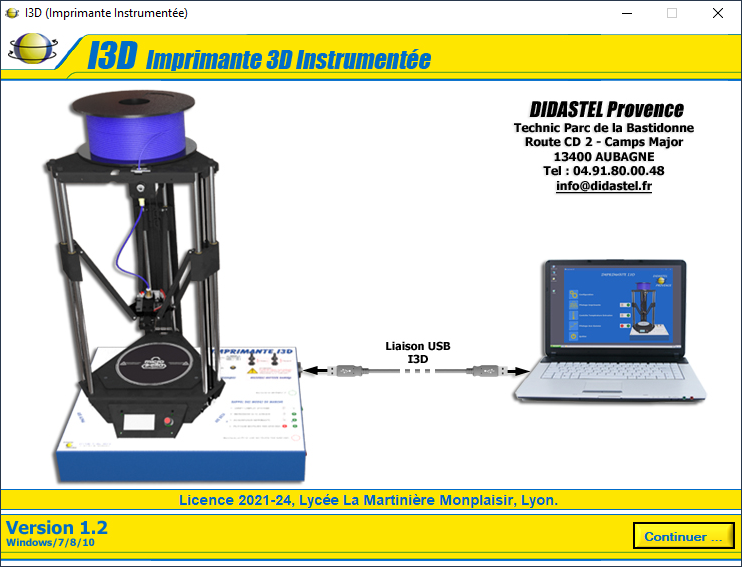
\includegraphics[width=.55\textwidth]{images/fig_00}
}%figues de la page de garde

\def\xxpied{%
Chirurgie mini-invasive robotisée\\
Concours Centrale Supelec -- PSI 2019%
}

\setcounter{secnumdepth}{5}
%---------------------------------------------------------------------------

\usepackage{bm}
\begin{document}
%\chapterimage{png/Fond_Cin}
\pagestyle{empty}


%%%%%%%% PAGE DE GARDE COURS
\ifcours
\begin{tikzpicture}[remember picture,overlay]
\node at (current page.north west)
{\begin{tikzpicture}[remember picture,overlay]
\node[anchor=north west,inner sep=0pt] at (0,0) {\includegraphics[width=\paperwidth]{\thechapterimage}};
\draw[anchor=west] (-2cm,-8cm) node [line width=2pt,rounded corners=15pt,draw=ocre,fill=white,fill opacity=0.6,inner sep=40pt]{\strut\makebox[22cm]{}};
\draw[anchor=west] (1cm,-8cm) node {\huge\sffamily\bfseries\color{black} %
\begin{minipage}{1cm}
\rotatebox{90}{\LARGE\sffamily\textsc{\color{ocre}\textbf{\xxnumpartie}}}
\end{minipage} \hfill
\begin{minipage}[c]{14cm}
\begin{titrepartie}
\begin{flushright}
\renewcommand{\baselinestretch}{1.1} 
\Large\sffamily\textsc{\textbf{\xxpartie}}
\renewcommand{\baselinestretch}{1} 
\end{flushright}
\end{titrepartie}
\end{minipage} \hfill
\begin{minipage}[c]{3.5cm}
{\large\sffamily\textsc{\textbf{\color{ocre} \discipline}}}
\end{minipage} 
 };
\end{tikzpicture}};
\end{tikzpicture}


\begin{tikzpicture}[overlay]
\node[shape=rectangle, 
      rounded corners = .25 cm,
	  draw= ocre,
	  line width=2pt, 
	  fill = ocre!10,
	  minimum width  = 2.5cm,
	  minimum height = 3cm,] at (18cm,0) {};
\node at (17.7cm,0) {\rotatebox{90}{\textbf{\Large\color{ocre}{\classe}}}};
%{};
\end{tikzpicture}

\vspace{3.5cm}

\begin{tikzpicture}[remember picture,overlay]
\draw[anchor=west] (-2cm,-6cm) node {\huge\sffamily\bfseries\color{black} %
\begin{minipage}{2cm}
\begin{center}
\LARGE\sffamily\textsc{\color{ocre}\textbf{\xxactivite}}
\end{center}
\end{minipage} \hfill
\begin{minipage}[c]{15cm}
\begin{titrechapitre}
\renewcommand{\baselinestretch}{1.1} 
\Large\sffamily\textsc{\textbf{\xxnumchapitre}}

\Large\sffamily\textsc{\textbf{\xxchapitre}}
\vspace{.5cm}

\renewcommand{\baselinestretch}{1} 
\normalsize\normalfont
\xxcompetences
\end{titrechapitre}
\end{minipage}  };
\end{tikzpicture}
\vfill

\begin{flushright}
\begin{minipage}[c]{.3\linewidth}
\begin{center}
\xxfigures
\end{center}
\end{minipage}\hfill
\begin{minipage}[c]{.6\linewidth}
\startcontents
\printcontents{}{1}{}
\end{minipage}
\end{flushright}

\begin{tikzpicture}[remember picture,overlay]
\draw[anchor=west] (4.5cm,-.7cm) node {
\begin{minipage}[c]{.2\linewidth}
\begin{flushright}

\includegraphics[width=2cm]{png/logoCC}
\end{flushright}
\end{minipage}
\begin{minipage}[c]{.2\linewidth}
\textsl{\xxauteur} \\
\textsl{\classe}
\end{minipage}
 };
\end{tikzpicture}
\newpage
\pagestyle{fancy}

\newpage
\pagestyle{fancy}

\else
\fi


%%%%%%%% PAGE DE GARDE TD
\iftd
\begin{tikzpicture}[remember picture,overlay]
\node at (current page.north west)
{\begin{tikzpicture}[remember picture,overlay]
\draw[anchor=west] (-2cm,-3.25cm) node [line width=2pt,rounded corners=15pt,draw=ocre,fill=white,fill opacity=0.6,inner sep=40pt]{\strut\makebox[22cm]{}};
\draw[anchor=west] (1cm,-3.25cm) node {\huge\sffamily\bfseries\color{black} %
\begin{minipage}{1cm}
\rotatebox{90}{\LARGE\sffamily\textsc{\color{ocre}\textbf{\xxnumpartie}}}
\end{minipage} \hfill
\begin{minipage}[c]{13.5cm}
\begin{titrepartie}
\begin{flushright}
\renewcommand{\baselinestretch}{1.1} 
\Large\sffamily\textsc{\textbf{\xxpartie}}
\renewcommand{\baselinestretch}{1} 
\end{flushright}
\end{titrepartie}
\end{minipage} \hfill
\begin{minipage}[c]{3.5cm}
{\large\sffamily\textsc{\textbf{\color{ocre} \discipline}}}
\end{minipage} 
 };
\end{tikzpicture}};
\end{tikzpicture}

%%%%%%%%%% PAGE DE GARDE TD %%%%%%%%%%%%%%%
\begin{tikzpicture}[overlay]
\node[shape=rectangle, 
      rounded corners = .25 cm,
	  draw= ocre,
	  line width=2pt, 
	  fill = ocre!10,
	  minimum width  = 2.5cm,
	  minimum height = 2.5cm,] at (18.5cm,0) {};
\node at (17.7cm,0) {\rotatebox{90}{\textbf{\Large\color{ocre}{\classe}}}};
%{};
\end{tikzpicture}

% PARTIE ET CHAPITRE
\begin{tikzpicture}[remember picture,overlay]
\draw[anchor=west] (-1cm,-2.1cm) node {\large\sffamily\bfseries\color{black} %
\begin{minipage}[c]{15cm}
\begin{flushleft}
\xxnumchapitre \\
\xxchapitre
\end{flushleft}
\end{minipage}  };
\end{tikzpicture}

% Bandeau titre exo
\begin{tikzpicture}[remember picture,overlay]
\draw[anchor=west] (-2cm,-6cm) node {\huge\sffamily\bfseries\color{black} %
\begin{minipage}{5cm}
\begin{center}
\LARGE\sffamily\color{ocre}\textbf{\textsc{\xxactivite}}

\begin{center}
\xxfigures
\end{center}

\end{center}
\end{minipage} \hfill
\begin{minipage}[c]{12cm}
\begin{titrechapitre}
\renewcommand{\baselinestretch}{1.1} 
\large\sffamily\textbf{\textsc{\xxtitreexo}}

\small\sffamily{\textbf{\textit{\color{black!70}\xxsourceexo}}}
\vspace{.5cm}

\renewcommand{\baselinestretch}{1} 
\normalsize\normalfont
\xxcompetences
\end{titrechapitre}
\end{minipage}  };
\end{tikzpicture}

\else
\fi


%%%%%%%% PAGE DE GARDE FICHE
\iffiche
\begin{tikzpicture}[remember picture,overlay]
\node at (current page.north west)
{\begin{tikzpicture}[remember picture,overlay]
\draw[anchor=west] (-2cm,-3.25cm) node [line width=2pt,rounded corners=15pt,draw=ocre,fill=white,fill opacity=0.6,inner sep=40pt]{\strut\makebox[22cm]{}};
\draw[anchor=west] (1cm,-3.25cm) node {\huge\sffamily\bfseries\color{black} %
\begin{minipage}{1cm}
\rotatebox{90}{\LARGE\sffamily\textsc{\color{ocre}\textbf{\xxnumpartie}}}
\end{minipage} \hfill
\begin{minipage}[c]{14cm}
\begin{titrepartie}
\begin{flushright}
\renewcommand{\baselinestretch}{1.1} 
\large\sffamily\textsc{\textbf{\xxpartie} \\} 

\vspace{.2cm}

\normalsize\sffamily\textsc{\textbf{\xxnumchapitre -- \xxchapitre}}
\renewcommand{\baselinestretch}{1} 
\end{flushright}
\end{titrepartie}
\end{minipage} \hfill
\begin{minipage}[c]{3.5cm}
{\large\sffamily\textsc{\textbf{\color{ocre} \discipline}}}
\end{minipage} 
 };
\end{tikzpicture}};
\end{tikzpicture}


\begin{tikzpicture}[overlay]
\node[shape=rectangle, 
      rounded corners = .25 cm,
	  draw= ocre,
	  line width=2pt, 
	  fill = ocre!10,
	  minimum width  = 2.5cm,
	  minimum height = 2.5cm,] at (18.5cm,0) {};
\node at (17.7cm,0) {\rotatebox{90}{\textbf{\large\color{ocre}{\classe}}}};
%{};
\end{tikzpicture}



\else
\fi



\vspace{4.5cm}
\pagestyle{fancy}
\thispagestyle{plain}


\def\columnseprulecolor{\color{ocre}}
\setlength{\columnseprule}{0.4pt} 

\section{Analyse des propriétés des signaux physiologiques}

\begin{obj}
Analyser les propriétés des signaux physiologiques et en déduire des éléments du cahier des charges
de la loi de commande pour assurer le déplacement du robot avec le niveau de précision requis.
\end{obj}

\subsection{Analyse des propriétés des signaux des mouvements physiologiques}

\begin{obj}
Proposer un algorithme permettant de mettre en évidence les propriétés des mouvements respiratoires.
\end{obj}
\subparagraph{} ~\\ %Q1
\textbf{Proposition 1}
En première approximation, on peut dire que ce signal est périodique, de période \SI{4,8}{s}. La valeur maximale est de \SI{5}{mm} et la valeur minimale est de \SI{-2,5}{s}.
Si on avait à la modéliser par un signal sinusoïdal on aurait $e(t)=3,75 \sin\left(\dfrac{2\pi}{4,8} t\right) + 1,25$.

\textbf{Proposition 2}

Le signal semble presque periodique même si les amplitudes des déplacement ne pas exactement les mêmes.
L'amplitude maximale obtenue est d'environ $\dfrac{5+2,3}{2}=\SI{3,65}{mm}$ et l'amplitude minimale obtenue est d'environ : $\dfrac{4+6}{2}=\SI{3}{mm}$;
La période des oscillation est d'environ $
T\approx\dfrac{41-4}{9}\approx \SI{4,1}{s}$. 
Soit une pulsation de $\omega\approx \SI{1,53}{rad.s^{-1}}$.


\subparagraph{} %Q2
D'après la définition, 
$\hat{S}\left( f_n\right)= \dfrac{1}{N_f} \sum \limits_{k=0}^{N_f-1} s\left[kT_e\right] \text{e}^{-i 2 \pi f_nT_e k}$

$= \dfrac{1}{N_f} \left(
 s\left[0 T_e\right] \text{e}^{-i 2 \pi f_nT_e 0} + 
 s\left[T_e\right] \text{e}^{-i 2 \pi f_nT_e } + ... 
 s\left[\left( N_f-1\right)T_e\right] \text{e}^{-i 2 \pi f_nT_e \left( N_f-1\right)}\right)$

$= \dfrac{1}{N_f} \left(
 s\left[0\right] + 
 s\left[T_e\right] \text{e}^{-i 2 \pi f_nT_e } + ... 
 s\left[\left( N_f-1\right)T_e\right] \text{e}^{-i 2 \pi f_nT_e \left( N_f-1\right)}\right)$.
 
 On a donc $l_k\left(f_n\right)=\dfrac{1}{N_f}\text{e}^{-i 2 \pi f_nT_e k}$.
 

\subparagraph{} %Q3

On a $L_n = \begin{pmatrix}  l_0 f_n  & l_1 f_n & l_2 f_n & \ldots & l_{N-1} f_n\end{pmatrix}$.
Par ailleurs, 
$S_p = 
\begin{pmatrix} \hat{S}\left( 0\right) \\ \hat{S}\left( f_1\right) \\ \hat{S}\left( f_2\right)  \\ \vdots \\ \hat{S}\left( f_{N-1}\right) \end{pmatrix} 
=
\begin{pmatrix} 
L_0 V_s \\
L_1 V_s \\
L_2 V_s \\
\vdots \\
 L_{N-1} V_s\end{pmatrix}$.

On a donc $ L_{k} V_s =\begin{pmatrix}  l_0 f_k  & l_1 f_k & l_2 f_k & \ldots & l_{N-1} f_k\end{pmatrix} \begin{pmatrix}
s[0]  \\ s[T_e] \\ s[2T_e] \\ \vdots \\ s\left[\left(N-1\right)T_e\right] \\   \end{pmatrix} = \sum  \limits_{i=0}^{N-1} l_i f_k s\left[i T_e\right]$.


Ainsi la matrice $M$ est composé de toutes les lignes $L_n$ pour $n\in  \llbracket 0,N_f-1\rrbracket$.

La matrice $M$ aura donc pour forme : 

\begin{align*}
M=\dfrac{1}{N_f}
\left(
\begin{array}{cccc}
1 & 1 & \ldots & 1 \\ 
1 & e^{-i2\pi f_1T_e} & \ldots & e^{-i2\pi f_{1}T_e(N-1)} \\ 
\vdots & e^{-i2\pi f_nT_e} & \ldots & e^{-i2\pi f_{n}T_e(N-1)} \\ 
1 & e^{-i2\pi f_{N_f-1}T_e} & \ldots & e^{-i2\pi f_{N_f-1}T_e(N-1)} \\ 
\end{array} 
\right)
\end{align*}



\subparagraph{} %Q4
De la question précédente, on peut exprimer le terme $a_{n,m}$ 
$a_{n,m}=\dfrac{1}{N_f}e^{-i2\pi f_{n}T_em}$.


\subparagraph{} %Q5

En posant 

$
X=-i2\pi
\left(
\begin{array}{c}
0\\
f_1\\
f_2\\
\vdots\\
f_{N_f-1}
\end{array}
\right)
\cdot
\left(
\begin{array}{ccccc}
0& T_e & 2T_e &\ldots & (N-1)T_e
\end{array}
\right)
=-i2\pi E_f\cdot t_k
$, on obtient bien, $
M=\dfrac{1}{N_f}\exp(X)$.

\subparagraph{} %Q6

\begin{python}
import numpy as np
def calculSpectre(Signal,Nf,fmax,Te):
    Vs=np.transpose([np.array(Signal)])
    Ef=np.transpose([np.linspace(0,fmax,Nf)])
    tk=np.array([range(len(Signal))])*Te
    X=np.dot(Ef,tk)*(-1j*2*np.pi)
    M=1/Nf*np.exp(X)
    Sp=np.dot(M,Vs)
    An=abs(Sp)
    return An
\end{python}

\subsection{Cahiers des charges partiel de la chaîne d'asservissement en position du robot esclave}

\begin{obj}
Déterminer une valeur numérique pour la bande passante de l’asservissement en position du robot
esclave et vérifier le cahier des charges associé.
\end{obj}

\subparagraph{}	

D'une part, $H(p)=\dfrac{\varepsilon (p)}{Z^*(p)}$ et d'autre part, $F(p)=\dfrac{Z (p)}{Z^*(p)}$. Enfin, $\varepsilon(p)=Z^*(p)-Z(p)$. On a donc $\varepsilon(p)=\dfrac{\varepsilon(p)}{H(p)} - F(p)Z^*(p)=\dfrac{\varepsilon(p)}{H(p)} - F(p)\dfrac{\varepsilon(p)}{H(p)}$. On a donc  $\varepsilon(p)=\dfrac{\varepsilon(p)}{H(p)} - F(p)\dfrac{\varepsilon(p)}{H(p)} \Leftrightarrow $ $H(p)=1 - F(p)= p\dfrac{p+2\xi\omega_0  }{p^2+2\xi\omega_0 p + \omega_0^2}$.


En mettant cette fonction de transfert sous forme canonique, on  obtient : 

$
H(p)=\dfrac{2\xi\cdot p}{\omega_0}\dfrac{1+\dfrac{p}{2\xi\omega_0}}{1+\dfrac{2\xi}{\omega_0}p+\dfrac{p^2}{\omega_0^2}}
$.

\begin{itemize}
\item Le module de cette fonction de transfert en remplaçant $p$ par $i\omega$ représente le rapport des amplitudes en régime permanent vis-à-vis d'une entrée $z*(t)$ sinusoïdale : 
$
\dfrac{\varepsilon_2}{A_2}=\Vert H(i\omega_2)\Vert
$.
\item L'argument de cette fonction de transfert en remplaçant $p$ par $i\omega$ représente le déphasage en régime permanent vis-à-vis d'une entrée $z^*(t)$ sinusoïdale : 
$
\Theta_2-\Phi_2=\arg\left(H(i\omega_2)\right)
$.
\end{itemize}

Ainsi on a : 
$
\left\{
\begin{array}{c}
\varepsilon_2=A_2\cdot \Vert H(i\omega_2)\Vert\\
\\
\Theta_2=\arg\left(H(i\omega_2)\right)+\Phi_2
\end{array}
\right.
$.


Supposons que  $z_2(t)=A_2\sin \left(\omega_2 t + \Phi_2 \right)$. De plus, $\varepsilon_2(t)=\varepsilon_2 \sin \left( \omega_2 t + \Theta_2 \right)$. On a donc, $\varepsilon_2 = || H\left( i\omega_2\right)|| A_2$, $\Phi_2 - \Theta_2 = \arg \left(H\left(i\omega_2\right)\right)$.




En considérant de faibles pulsations telles que $\omega\ll \omega_0$, on peut effectuer l'approximation : 
$
H(p)\approx \dfrac{2\xi\cdot p}{\omega_0}
$.

On obtient donc bien : 
$
\Vert H(i\omega)\Vert\approx K\cdot \omega
$ 
avec $K=\dfrac{2\xi}{\omega_0}$.

\textbf{Remarque }: il aurait sûrement été préférable de préciser ici au candidat qu'on a $z_n(t)=A_n\sin \left(2\pi f_n t + \Phi_n \right)=A_n\sin \left(\omega_n t + \Phi_n \right)$. 

\subparagraph{}	
Lorsque $\omega << \omega_0$, $\left|\left|  \dfrac{1}{p^2+2\xi\omega_0 p + \omega_0^2} \right|\right|$ tend vers 0. Calculons $\left|\left|  \left( j \omega \right) ^2+2\xi\omega_0  \omega j  \right|\right| =\sqrt{4\xi^2\omega_0^2 \omega^2 + \omega^2} =\omega \sqrt{4\xi^2\omega_0^2  + 1}$. 

On a donc $|| H\left( i\omega\right)|| \simeq K\omega $ avec $K=\sqrt{4\xi^2\omega_0^2  + 1}$ lorsque $\omega << \omega_0$.

\textcolor{red}{A VERIFIER Au final, $\varepsilon_2 \simeq \omega_2 \sqrt{4\xi^2\omega_0^2  + 1} A_2\sin \left(\omega_2 t + \Phi_2 \right) $.}

\subparagraph{}	~\\
D'après l'exigence 1.3.3, $\dfrac{\varepsilon_2}{A_2}<10^{-2}$, on obtient alors la relation suivante : $
\dfrac{\varepsilon_2}{A_2}\approx \dfrac{2\xi\omega_2}{\omega_0}<10^{-2}$.  \textcolor{red}{XP : Pourquoi ?}

Ce qui donne $\omega_0>200\xi\omega_2\approx \SI{603}{rad.s^{-1}}$

D'après le cahier des charges l'exigence 1.2 concernant l'asservissement en position, et donc la fonction de transfert $F(p)$, impose une bande passante (que l'on suppose à $\SI{0}{dB}$), inférieure à $\SI{30}{rad.s^{-1}}$. $F(p)$ est une fonction de transfert du second ordre de gain 1 et la bande passante à $\SI{0}{dB}$ est de l'ordre de $\omega_0\approx \SI{600}{rad.s^{-1}}$. \textbf{Le cahier des charges est donc bien respecté.}


% Piste 2 Calculons $\omega_{BP}$ tel que $||F\left(j\omega_{BP}\right)|| = 0$ : 
%$\left|\left|F\left(j\omega\right)\right|\right|$ 
%$=\left|\left| \dfrac{\omega_0^2}{\omega_0^2-\omega^2+2\xi\omega_0\omega j} \right|\right|$

% $=\left|\left| 
% \dfrac{
% \omega_0^2 \left(\omega_0^2-\omega^2-2\xi\omega_0\omega j \right)
% }{
% \left( \omega_0^2-\omega^2+2\xi\omega_0\omega j\right) \left(\omega_0^2-\omega^2-2\xi\omega_0\omega j\right)}  % \right|\right|$
% $=\left|\left| 
% \dfrac{
% \omega_0^2 \left(\omega_0^2-\omega^2-2\xi\omega_0\omega j \right)
% }{
%  \left(\omega_0^2-\omega^2\right)^2 +4\xi^2\omega_0^2\omega^2 
% }  \right|\right|$

% Piste 1Supposons que $\dfrac{\varepsilon_2}{A_2} < 10^{-2}$ (exigence 1.3.2), on a alors $  \sqrt{4\xi^2\omega_0^2  + 1} \sin \left(\omega_2 t + \Phi_2 \right) < 10^{-2} $ 
% $\Rightarrow  \sqrt{4\omega_0^2  + 1} \sin \left(\omega_2 t + \Phi_2 \right) < 10^{-2} $.

\textbf{Remarque :} je ne comprends pas bien la formulation de la question : << En considérant $\varepsilon_2$, déterminer (...) >>.


\section{Analyse géométrique et élaboration du modèle dynamique du robot esclave}

\begin{obj}
Vérifier la capabilité du robot esclave à respecter le cahier des charges et déterminer le modèle dynamique
d’un des axes du robot esclave utilisé pour dimensionner sa commande.
\end{obj}

\subsection{Vérification de la capabilité du robot esclave}
\begin{obj}
Vérifier la capacité du robot esclave à respecter l’exigence de précision 1.3.3 et dimensionner les
capteurs installés sur le robot en conséquence.
\end{obj}


\subparagraph{}%10	

D'après le cahier des charges $\varepsilon_r<1\%$. 
D'après la figure 4, la variation maximale des déplacement est de $\SI{7,5}{mm}$. Il faudrait donc une résolution de $s_{\text{max}}=\SI{75}{\mu m}$


\textcolor{red}{XP : Je ne vois pas comment déterminer la résolution à partir de la courbe. Pb de l'exigence 1.2.1 avec la précision de $\SI{10}{\mu m}$.}

\subparagraph{}%11
On a $\lambda(t)=\lambda_0 + \dfrac{p}{2\pi} \theta_{83}$. 
En conséquences, $\vect{BD}=\vect{BC}+\vect{CD}=l_3\vect{y_3}+\lambda(t)\vect{z_3}+l_4\vect{z_4}
=l_3\vect{y_3}+\left( \lambda_0 + \dfrac{p}{2\pi} \theta_{83} \right)\vect{z_3}+l_4\vect{z_3}$.


\subparagraph{}%12
%En projetant $\vect{BD}$ dans la base $\base{x_2'}{y_2'}{z_2'}$, on a 
% $\vect{BD}=l_3\vect{y_3}+\left( \lambda_0 + \dfrac{p}{2\pi} \theta_{83} \right)\vect{z_3}+l_4\vect{z_3}$
% $ =l_3\left( \cos \theta_{32} \vect{x_2'} + \sin\theta_{32} \vect{y_2'}  \right)+\left( \lambda_0 + \dfrac{p}{2\pi} \theta_{83} +l_4\right)\vect{z_2'}$.

% Avec l'hypothèse que $\theta_{32}$ reste petit, on a  $\vect{BD}=l_3\left(  \vect{x_2'} + \theta_{32} \vect{y_2'}  \right)+\left( \lambda_0 + \dfrac{p}{2\pi} \theta_{83} +l_4\right)\vect{z_2'}$.

%  Ainsi, $\left(x_D,y_D,z_D\right)=
%\left( l_3,l_3 \theta_{32}, \lambda_0 + \dfrac{p}{2\pi} \theta_{83} +l_4\right)$.

En projetant $\vect{BD}$ dans la base $\base{x_2'}{y_2'}{z_2'}$, on a 
 $\vect{BD}=l_3\vect{y_3}+\left( \lambda_0 + \dfrac{p}{2\pi} \theta_{83} \right)\vect{z_3}+l_4\vect{z_3}$
 $ =l_3\left( \cos \theta_{32} \vect{y_2'} - \sin\theta_{32} \vect{x_2'}  \right)+\left( \lambda_0 + \dfrac{p}{2\pi} \theta_{83} +l_4\right)\vect{z_2'}$.
 
 Avec l'hypothèse que $\theta_{32}$ reste petit, on a  $\vect{BD}=l_3\left(  \vect{y_2'} - \theta_{32} \vect{x_2'}  \right)+\left( \lambda_0 + \dfrac{p}{2\pi} \theta_{83} +l_4\right)\vect{z_2'}$.
  Ainsi,
  
  $\left(x_D,y_D,z_D\right)=
\left(-l_3 \theta_{32},l_3, \lambda_0 + \dfrac{p}{2\pi} \theta_{83} +l_4\right)$. \textcolor{red}{XP : et $\lambda_0$ ?}

\subparagraph{}%13

Soit, $s_D=3\sqrt{s_X^2+s_Y^2+s_Z^2}$. Par calcul différentiel :  \textcolor{red}{XP?}

\begin{minipage}{0.5\textwidth}
\begin{align*}
\left\{
\begin{array}{c}
dx_D=-l_3d\theta_{32}\\
dy_D=0\\
dz_D=\dfrac{p}{2\pi}d\theta_{83}
\end{array}
\right.
\end{align*}
\end{minipage}
\begin{minipage}{0.5\textwidth}

\begin{align*}
\left\{
\begin{array}{c}
s_X=\Delta x_D=-l_3\Delta \theta_{32}=-l_3 s_{\text{capteur}}\\
s_Y=\Delta y_D=0\\
s_Z=\Delta z_D=\dfrac{p}{2\pi}\Delta \theta_{83}=\dfrac{p}{2\pi}s_{\text{capteur}}
\end{array}
\right.
\end{align*}
\end{minipage}

Ainsi,$
s_D=3\cdot s_{\text{capteur}}\sqrt{l_3^2+\dfrac{p^2}{4\pi^2}}
$.
Le cahier des charges impose la relation suivante,$
s_{\text{capteur}}<\dfrac{75\mu m}{3\sqrt{l_3^2+\dfrac{p^2}{4\pi^2}}}
$.

L'application numérique donne $s_{\text{capteur}}=2,72\times \SI{e-5}{mm}$. Le cahier des charges est bien respecté.


\subsection{Détermination et vérification du modèle dynamique du robot esclave}
\begin{obj}
Déterminer le modèle dynamique du robot esclave en vue de l’élaboration de sa commande.
\end{obj}

\subparagraph{}%14
On se place en régime permanent. Le rendement peut s'exprimer par 
$\eta_9 =\dfrac{C_{73}\dot{\theta}_{32}}{C_{m2}\dot{\theta}_{72}}=\dfrac{C_{73}}{C_{m2}}r_9$. 
On a donc, en régime permanent, $\vect{C_{73}}=C_{73}\vect{z'_2}=C_{m2}\dfrac{\eta_9}{r_9}\vect{z'_2}$.


\subparagraph{}%15
Au vu du tracé expérimental de $C_{73}$ en fonction de $C_{m2}$, on peut réaliser une linéarisation sur l'intervalle $[0,10]$ et $C_{73}\simeq 3 C_{m2}$. 
D'après les données constructeur, on a $C_{73}=C_{m2}\dfrac{\eta_9}{r_9}=C_{m2}\dfrac{0,78}{0,25}=\SI{3,12}{Nm}$.

On peut donc valider les valeurs données par le constructeur.
\subsection{Élaboration du modèle dynamique d’un axe du robot esclave}


\subparagraph{}%16
\begin{center}
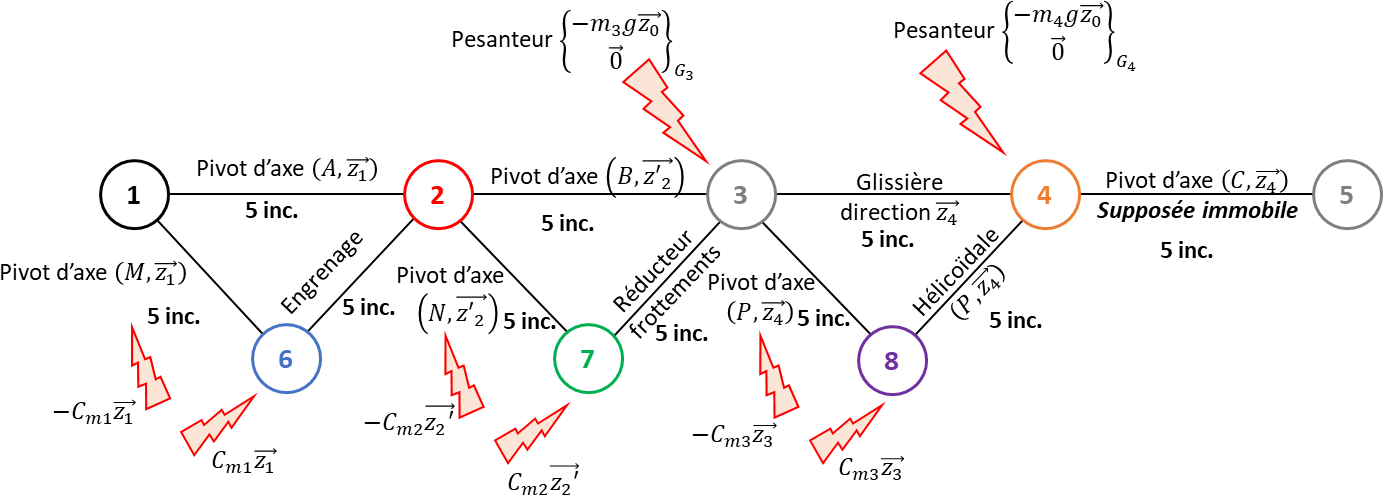
\includegraphics[width=\textwidth]{images/fig_02}
\end{center}
%
%\begin{center}
%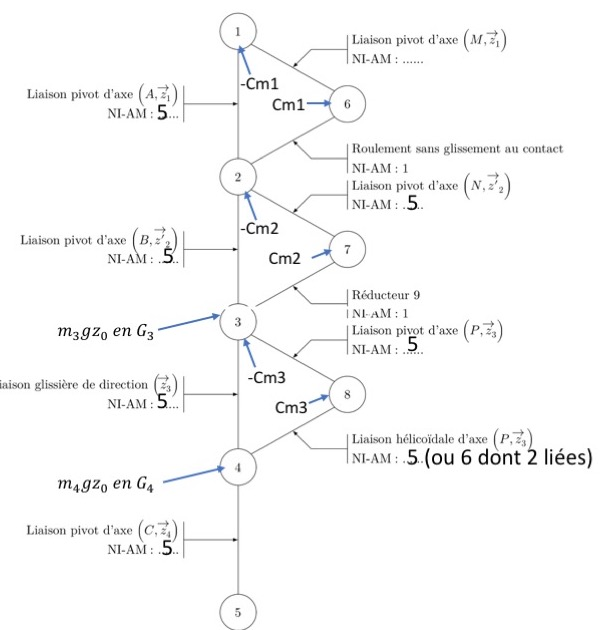
\includegraphics[width=0.8\textwidth]{images/graphe_structure_complet.jpg}
%\end{center}
\subparagraph{}%17
On cherche à déterminer le couple $C_{m2}$ à fournir sur l'arbre 7. L'arbre 7 est en rotation autour de l'axe $\axe{N}{z_2'}$. Il entraîne l'ensemble $\left\{3+8+4+5\right\}$ en rotation autour de l'axe $\axe{B}{z_2'}$.

\begin{center}
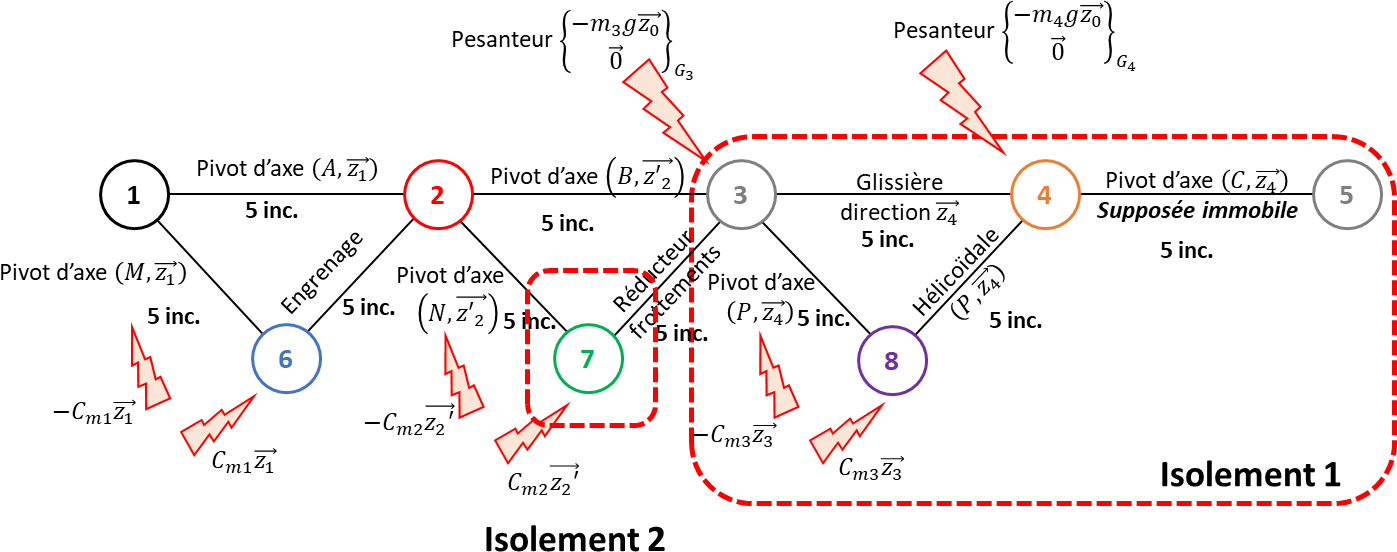
\includegraphics[width=\textwidth]{images/fig_05}
\end{center}

On propose donc les isolements et des théorèmes associés suivants : 
\begin{itemize}
\item isolement de $\left\{3+8+4+5\right\}$ : théorème du moment dynamique en projection sur $\left(B,\overrightarrow{z}_2'\right)$ qui permet de relier l'action de 7 sur 3 aux paramètres de mouvement de l'ensemble $\left\{3+8+4+5\right\}$ qui représente dans le cas particulier du mouvement souhaité la même classe d'équivalence;
\item isolement de $7$ : théorème du moment dynamique selon $\left(N,\overrightarrow{z}_2'\right)$ qui revient à un théorème du moment statique car l'inertie de 7 est négligeable. Cela permet de relier $C_{m2}$ à l'action de 3 sur 7.
\end{itemize}
Cet isolement permet de ne pas faire apparaître les inconnues dans les liaisons pivot entre 2 et 7 ainsi qu'entre 7 et 3. 
\subparagraph{}%18
On cherche $\vectv{G_4}{4}{1}$. On a $\vect{OG_4}=\vect{OA}+\vect{AB}+\vect{BC}+\vect{CG_4}$ $=l_0\vect{y_0}+l_1\vect{y_1}+l_2\vect{y_2}+l_2'\vect{y_2'}+l_3\vect{y_3}+\lambda(t)\vect{z_3}+b_4\vect{z_4}$.
On a $\alpha_1=\dfrac{\pi}{4}$ et $\alpha_2=-\dfrac{\pi}{4}$.

On a donc $\vectv{G_4}{4}{1}= \left[\dfrac{\dd \vect{OG_4}}{\dd t}\right]_{\rep{0}} $ 

$= 
\left[\dfrac{\dd l_0\vect{y_0}}{\dd t}\right]_{\rep{0}}+
\left[\dfrac{\dd l_1\vect{y_1}}{\dd t}\right]_{\rep{0}}+
\left[\dfrac{\dd l_2\vect{y_2}}{\dd t}\right]_{\rep{0}}+
\left[\dfrac{\dd l_2'\vect{y_2'}}{\dd t}\right]_{\rep{0}}+
\left[\dfrac{\dd l_3\vect{y_3}}{\dd t}\right]_{\rep{0}}+
\left[\dfrac{\dd \lambda(t)\vect{z_3}}{\dd t}\right]_{\rep{0}}+
\left[\dfrac{\dd b_4\vect{z_4}}{\dd t}\right]_{\rep{0}}$

$= 
\vect{0}+
\vect{0}+
l_2\left[\dfrac{\dd \vect{y_2}}{\dd t}\right]_{\rep{0}}+
l_2'\left[\dfrac{\dd \vect{y_2'}}{\dd t}\right]_{\rep{0}}+
l_3\left[\dfrac{\dd \vect{y_3}}{\dd t}\right]_{\rep{0}}+
\lambda(t)\left[\dfrac{\dd \vect{z_3}}{\dd t}\right]_{\rep{0}}+
\dot{\lambda}(t)\left[\dfrac{\dd \vect{z_3}}{\dd t}\right]_{\rep{0}}+
b_4\left[\dfrac{\dd \vect{z_4}}{\dd t}\right]_{\rep{0}}$

$= 
l_2\left[ \vecto{2}{0} \wedge \vect{y_2} \right]+
l_2'\left[ \vecto{2'}{0} \wedge \vect{y_2'} \right]+
l_3\left[ \vecto{3}{0} \wedge \vect{y_3} \right]+
\lambda(t)\left[ \vecto{3}{0} \wedge \vect{z_3} \right]+
\dot{\lambda}(t)\vect{z_3}+
b_4\left[ \vecto{4}{0} \wedge \vect{z_4} \right]$. 

$= 
l_2\left[ \dot{\theta}_{21}\vect{z_2} \wedge \vect{y_2} \right]+
l_2'\left[ \dot{\theta}_{21}\vect{z_2} \wedge \vect{y_2'} \right]+
l_3\left[ \left(\dot{\theta}_{21}\vect{z_2}+\dot{\theta}_{32}\vect{z_3} \right) \wedge \vect{y_3} \right]+
\lambda(t)\left[ \left(\dot{\theta}_{21}\vect{z_2}+\dot{\theta}_{32}\vect{z_3} \right) \wedge \vect{z_3} \right]+
\dot{\lambda}(t)\vect{z_3}+
b_4\left[ \left(\dot{\theta}_{21}\vect{z_2}+\dot{\theta}_{32}\vect{z_3} \right) \wedge \vect{z_3} \right]$. 

Or $\dot{\theta}_{21}=0$. On a donc :
$\vectv{G_4}{4}{1}= 
l_3\left(\dot{\theta}_{32}\vect{z_3} \wedge \vect{y_3} \right)+
\dot{\lambda}(t)\vect{z_3} =
-\dot{\theta}_{32}l_3\vect{x_3}  + \dot{\lambda}(t)\vect{z_3}$.

%
%$= 
%-l_2 \dot{\theta}_{21}\vect{x_2} 
%-l_2'\dot{\theta}_{21}\cos \alpha_2\vect{x_2}+
%l_3\left[ \dot{\theta}_{21}\vect{z_2}\wedge \vect{y_3}-\dot{\theta}_{32}\vect{x_3}  \right]+
%\lambda(t) \dot{\theta}_{21}\sin \alpha_2\vect{x_2} +
%\dot{\lambda}(t)\vect{z_3}+ b_4\dot{\theta}_{21}\sin \alpha_2\vect{x_2}$. 
%
%
%Par ailleurs, 
%$\vect{z_2}\wedge \vect{y_3}=\vect{z_2}\wedge \left( \cos \theta_{32} \vect{y_2'} -\sin \theta_{32} \vect{x_2'}  \right)$
%$= \cos \theta_{32} \vect{z_2}\wedge  \vect{y_2'} -\sin \theta_{32} \vect{z_2}\wedge\vect{x_2'}  $
%$= -\cos \theta_{32} \cos \alpha_2 \vect{x_2'} -\sin \theta_{32} \vect{y_2}  $.
%
%Au final, on a 
%
%$\vectv{G_4}{4}{1}=
%-l_2 \dot{\theta}_{21}\vect{x_2} 
%-l_2'\dot{\theta}_{21}\cos \alpha_2\vect{x_2}+
%l_3\left[ \dot{\theta}_{21}\left(-\cos \theta_{32} \cos \alpha_2 \vect{x_2'} -\sin \theta_{32} \vect{y_2}  \right)-\dot{\theta}_{32}\vect{x_3}  \right]+
%\lambda(t) \dot{\theta}_{21}\sin \alpha_2\vect{x_2} +
%\dot{\lambda}(t)\vect{z_3}+ b_4\dot{\theta}_{21}\sin \alpha_2\vect{x_2}$.
%

%En tenant compte de l'hypothèse $\dot{\theta}_{21}=0$, on a : $\vectv{G_4}{4}{1}=
%-\dot{\theta}_{32}l_3\vect{x_3}  + \dot{\lambda}(t)\vect{z_3}$.


\subparagraph{}%19
En utilisant l'évolution de $\dot{\theta}_{32}$, on peut déterminer le déplacement angulaire effectué en traçant l'aire sous la courbe :
$\theta_{32}=\dfrac{1}{2}\left( 1+0,5\right)\times 0,075 =\SI{0,056}{rad}\simeq 3^{\text{o}}$.

Cet angle étant faible, on peut donc considérer que $\forall t \cos \left(\theta_{32}(t)\right)\simeq 1$ et $\sin\left(\theta_{32}(t)\right)\simeq 0$.

\subparagraph{}%20

On donne $J_4$ le moment d'inertie du bras 4 autour de l'axe $\axe{G_4}{z_4}$.

\textbf{Méthode}
\begin{enumerate}
\item Expression de $\vectmd{B}{4}{1}\cdot\vect{z_4} = \left( \vectmd{G_4}{4}{1} + \vect{BG_4}\wedge m_4 \vectg{G_4}{4}{1}\right)\cdot\vect{z_4}$.
\item Calcul de $\vectmd{G_4}{4}{1}$.
\end{enumerate}

$\vectmd{G_4}{4}{1} \cdot\vect{z_4} = \left[ \dfrac{\dd \vectmc{G_4}{4}{1}}{\dd t} \right]_{\rep{0}}\cdot\vect{z_4}
=\left[ \dfrac{\dd \vectmc{G_4}{4}{1}\cdot \vect{z_4}}{\dd t} \right]-\vectmc{G_4}{4}{1}\cdot\left[ \dfrac{\dd \vect{z_4}}{\dd t} \right]_{\rep{0}}$



On a $\vectmc{G_4}{4}{1} =\inertie{G_4}{4} \vecto{4}{1}$ avec $\vecto{4}{1}=\underbrace{\vecto{4}{3}}_{\vect{0}}+\vecto{3}{2}+\vecto{2}{1} =\dot{\theta}_{32} \vect{z_3}+\underbrace{\dot{\theta}_{21}}_{0} \vect{z_2}=\dot{\theta}_{32} \vect{z_4}$.

Donc,
$\vectmc{G_4}{4}{1}\cdot\vect{z_4}=J_4\dot{\theta}_{32} $.

De plus, $ \left[ \dfrac{ \dd \vect{z_4}}{\dd t} \right]_{\rep{0}} = \vect{0} $. 
En conséquences, $\vectmd{G_4}{4}{1} \cdot\vect{z_4}  = J_4\ddot{\theta}_{32}$.

Par ailleurs, $\vectg{G_4}{4}{1}= \left[\dfrac{\dd \vectv{G_4}{4}{1}}{\dd t} \right]_{\rep{0}}=\left[\dfrac{\dd \left( -\dot{\theta}_{32}l_3\vect{x_3}  + \dot{\lambda}(t)\vect{z_3} \right)}{\dd t} \right]_{\rep{0}}$
$= -\ddot{\theta}_{32}l_3\vect{x_3} -\dot{\theta}_{32}l_3    \left(\dot{\theta}_{32} \vect{z_3}\wedge \vect{x_3} \right)  + \ddot{\lambda}(t)\vect{z_3}  $

$= -\ddot{\theta}_{32}l_3\vect{x_3} -l_3   \dot{\theta}_{32}^2  \vect{y_3} + \ddot{\lambda}(t)\vect{z_3}  $.

$\left(\vect{BG_4}\wedge m_4 \vectg{G_4}{4}{1}\right)\cdot\vect{z_4} = 
m_4\left( \left(l_3 \vect{y_3} + \lambda(t) \vect{z_3}+ b_4 \vect{z_4}\right) \wedge  \left(-\ddot{\theta}_{32}l_3\vect{x_3} -l_3   \dot{\theta}_{32}^2  \vect{y_3} + \ddot{\lambda}(t)\vect{z_3} \right) \right)\cdot \vect{z_{4,3}}$

Par simplification avec les propriétés du produit mixte et du produit vectoriel,

$
\left(\vect{BG_4}\wedge m_4 \vectg{G_4}{4}{1}\right)\cdot\vect{z_4} =
m_4\left( \left(l_3 \vect{y_3} \right) \wedge  \left(-\ddot{\theta}_{32}l_3\vect{x_3} \right) \right)\cdot \vect{z_{4,3}}
=m_4\cdot l_3^2\ddot{\theta}_{32}
$


  Au final,  $\vectmd{B}{4}{1}\cdot\vect{z_4} = J_4 \ddot{\theta}_{32}+\ddot{\theta}_{32}l_3^2 m_4 $.
  



%
%$= m_4\left( \left(l_3 \vect{y_3} + \lambda(t) \vect{z_3}+ b_4 \vect{z_4}\right) \wedge  \left(-\ddot{\theta}_{32}l_3\vect{x_3}\right)  + \left(l_3 \vect{y_3} + \lambda(t) \vect{z_3}+ b_4 \vect{z_4}\right) \wedge  \left(-l_3   \dot{\theta}_{32}^2  \vect{y_3}\right) + \left(l_3 \vect{y_3} + \lambda(t) \vect{z_3}+ b_4 \vect{z_4}\right) \wedge  \left(\ddot{\lambda}(t)\vect{z_3}\right) \right) \cdot \vect{z_4}$
%
%$= m_4\left(\left( \left(l_3 \vect{y_3} + \lambda(t) \vect{z_3}+ b_4 \vect{z_4}\right) \wedge  \left(-\ddot{\theta}_{32}l_3\vect{x_3}\right) \right) \cdot \vect{z_4} 
% + \left(\left(l_3 \vect{y_3} + \lambda(t) \vect{z_3}+ b_4 \vect{z_4}\right) \wedge  \left(-l_3   \dot{\theta}_{32}^2  \vect{y_3}\right)\right) \cdot \vect{z_4}
%  +\left( \left(l_3 \vect{y_3} + \lambda(t) \vect{z_3}+ b_4 \vect{z_4}\right) \wedge  \left(\ddot{\lambda}(t)\vect{z_3}\right) \right) \cdot \vect{z_4}\right)$
%  
%$= m_4\left(\left( \vect{z_4} \wedge  \left(l_3 \vect{y_3} + \lambda(t) \vect{z_3}+ b_4 \vect{z_4}\right)  \right) \cdot  \left(-\ddot{\theta}_{32}l_3\vect{x_3}\right)
% + \left(\vect{z_4} \wedge \left(l_3 \vect{y_3} + \lambda(t) \vect{z_3}+ b_4 \vect{z_4}\right)  \right) \cdot \left(-l_3   \dot{\theta}_{32}^2  \vect{y_3}\right)
%  +\left( \vect{z_4} \wedge \left(l_3 \vect{y_3} + \lambda(t) \vect{z_3}+ b_4 \vect{z_4}\right) \right) \cdot   \left(\ddot{\lambda}(t)\vect{z_3}\right) \right)$
%  
%  $= m_4\left(\left( \vect{z_4} \wedge  l_3 \vect{y_3}  \right) \cdot  \left(-\ddot{\theta}_{32}l_3\vect{x_3}\right)   \right)$
%
%  $= \ddot{\theta}_{32}l_3^2 m_4 $.
  



\subparagraph{}%21


Par analogie avec la question précédente, on a $\vectmd{B}{3}{1}\cdot\vect{z_4}= J_3\ddot{\theta}_{32}+\ddot{\theta}_{32}a_3^2 m_3$.

En conséquence,  $\vectmd{B}{3+4+5+8}{1}\cdot\vect{z_4} = \left(J_3+J_4\right) \ddot{\theta}_{32}+\ddot{\theta}_{32}\left( a_3^2 m_3  +l_3^2 m_4  \right)$.


\textcolor{red}{XP :il me semble que pour traiter la question serieusement il faudrait définir << proprement >> l'action de 3 sur 7}


\textbf{On isole l'ensemble $\{3,4,5,8\}$.}


\begin{itemize}
\item On réalise le bilan des actions mécaniques extérieures. 
\begin{itemize}
\item \textcolor{red}{ XP : La pesanteur crée un moment en $B$ suivant  $\vect{z_0}$ (le schéma est trompeur)}.
\item Action de la pesanteur sur 3 : 
$\vectm{B}{\text{pes}}{3}\cdot \vect{z_4} $ $ =\left(\vect{BG_3}\wedge \left(-m_3g \vect{z_0}\right) \right)\vect{z_4}$ 
$ =\left(\left( a_3\vect{y_3} + b_3\vect{z_3}  \right)\wedge \left(-m_3g \vect{z_0}\right)\right)\vect{z_4}$
$ =\left( a_3\vect{y_4} \wedge \left(-m_3g \vect{z_0}\right)\right)\vect{z_4}$
$ =\left( \vect{z_4} \wedge a_3\vect{y_4}\right)\cdot  \left(-m_3g \vect{z_0}\right)$
$ = a_3 m_3g \left( \vect{x_3}\cdot \vect{z_0} \right)$
$ = a_3 m_3g \left(  \cos\theta_{32} \vect{x_2'} +\sin\theta_{32} \vect{y_2'} \right)\cdot \vect{z_0} $

On utilise les hypothèses de linéarisation vues précédemment et on a 
$\vectm{B}{\text{pes}}{3}\cdot \vect{z_4}= a_3 m_3g \vect{x_2'} \cdot \vect{z_0} $ 
$= a_3 m_3g \vect{x_2} \cdot \vect{z_0} $
$= a_3 m_3g \left( \cos \theta_{21} \vect{x_1} +\sin \theta_{21} \vect{y_1} \right)\cdot \vect{z_0} $
$= a_3 m_3g \left( \cos \theta_{21} \vect{x_0} +\sin \theta_{21}  \left( \cos \alpha_1 \vect{y_0} + \sin \alpha_1 \vect{z_0} \right) \right)\cdot \vect{z_0} $
$= a_3 m_3g \sin \theta_{21}   \sin \alpha_1    $. En faisant l'application numérique, on a donc 
$\vectm{B}{\text{pes}}{3}\cdot \vect{z_4}= a_3 m_3g  \dfrac{\sqrt{2}}{2} \dfrac{\sqrt{3}}{2}$

\item Action de la pesanteur sur 4 : 
$\vectm{B}{\text{pes}}{4}\cdot \vect{z_4} $ $ =\left(\vect{BG_4}\wedge \left(-m_4g \vect{z_0}\right) \right)\vect{z_4}$ 

$ =\left(\left(l_3\vect{y_3} + \lambda(t) \vect{z_3} + b_4\vect{z_4} \right)\wedge \left(-m_4g \vect{z_0}\right) \right)\vect{z_4}$. 

\textbf{Pour Emilien }
$
\left(\vect{BG_4}\wedge \left(-m_4g \vect{z_0}\right) \right)\vect{z_{4,3}}
=\overrightarrow{z}_3\wedge l_3\overrightarrow{y}_3\cdot \left(-m_4\cdot g\cdot \overrightarrow{z}_0\right)=m_4l_3g\overrightarrow{x}_3\cdot \overrightarrow{z}_0
$

Or,

$\overrightarrow{x}_3=\cos\theta_{32}\overrightarrow{x}_{2,2'}+\sin\theta_{32}\overrightarrow{y}_{2'}$

avec $\cos\theta_{32}\approx 1$ et $\sin\theta_{32}\approx 0$

 Donc, 
 
 $\overrightarrow{x}_3\cdot \overrightarrow{z}_0=\left(\cos\theta_{21}\overrightarrow{x}_{1,0}+\sin\theta_{21}\overrightarrow{y}_1\right)\cdot \overrightarrow{z}_0=\cos\theta_{21}\sin\alpha_1=\dfrac{\sqrt{2}}{4}$
 On obtient alors,
 
 $\vectm{B}{\text{pes}}{4}\cdot \vect{z_4} = l_3 m_4g  \dfrac{\sqrt{2}}{4}$.

\textbf{Pour Xavier : }

Par analogie avec le calcul précédent, $\vectm{B}{\text{pes}}{4}\cdot \vect{z_4} = l_3 m_4g  \dfrac{\sqrt{2}}{2} \dfrac{\sqrt{3}}{2} $.

%$ = a_3 m_3g \left(  \cos\theta_{32} \vect{x_2} +\sin\theta_{32} \left(\cos\alpha_{2} \vect{y_2} +\sin\alpha_{2} \vect{z_2}\right) \right)\cdot \vect{z_0} $

%$ = a_3 m_3g \left(  \cos\theta_{32} \left( \cos \theta_{21} \vect{x_1} +\sin \theta_{21} \vect{y_1} \right) +\sin\theta_{32} \left(\cos\alpha_{2} \left( \cos \theta_{21} \vect{y_1} -\sin \theta_{21} \vect{x_1} \right) +\sin\alpha_{2} \vect{z_1}\right) \right)\cdot \vect{z_0} $

%$ = a_3 m_3g \left(  \cos\theta_{32} \left( \cos \theta_{21} \vect{x_0} +\sin \theta_{21} \left( \cos \alpha_1 \vect{y_0} + \sin \alpha_1 \vect{z_0} \right) \right) +\sin\theta_{32} \left(\cos\alpha_{2} \left( \cos \theta_{21} \left( \cos \alpha_1 \vect{y_0} + \sin \alpha_1 \vect{z_0} \right)  -\sin \theta_{21} \vect{x_0} \right) +\sin\alpha_{2}  \left( \cos \alpha_1 \vect{z_0} - \sin \alpha_1 \vect{y_0} \right)  \right) \right)\cdot \vect{z_0} $

%$ = a_3 m_3g \left(  \cos\theta_{32} \left( \sin \theta_{21} \left(  \sin \alpha_1 \vect{z_0} \right) \right) +
%\sin\theta_{32} \left(\cos\alpha_{2} \left( \cos \theta_{21} \left( \sin \alpha_1 \vect{z_0} \right)  \right) +\sin\alpha_{2}  %\left( \cos \alpha_1 \vect{z_0}  \right)  \right) \right)\cdot \vect{z_0} $. 

\item $\vectm{B}{2}{3}\cdot \vect{z_0}=0$.
\item $\vectm{B}{7}{3}\cdot \vect{z_4}=C_{73}$ (Indication du sujet).
\end{itemize}
\item En appliquant le théorème du moment dynamique en $B$ en projection sur $\vect{z}$ on a donc 
$ C_{73} =  \left(J_3+J_4\right) \ddot{\theta}_{32}+\ddot{\theta}_{32}\left( a_3^2 m_3  +l_3^2 m_4  \right) + g  \dfrac{\sqrt{6}}{4} \left( a_3 m_3 + l_3 m_4\right) $.
\end{itemize}

\textbf{Il semblerait que ce qui est attendu soit d'utiliser ${C_{73}}=C_{m2}\dfrac{\eta_9}{r_9}$, mais cette relation avait été établie en régime permanent ce qui n'est plus le cas. } 


\textbf{Selon Xavier}
$ C_{m2}\dfrac{\eta_9}{r_9}=  \left(J_3+J_4  + a_3^2 m_3  +l_3^2 m_4 \right) \ddot{\theta}_{32} + g  \sin \theta_{21}   \sin \alpha_1 \left( a_3 m_3 + l_3 m_4\right) $.

Par identification, on a donc :
\begin{itemize}
\item $J_{eq} = J_3+J_4  + a_3^2 m_3  +l_3^2 m_4$;
\item $A  =\dfrac{\eta_9}{r_9}$;
\item $C_r(t)=-g  \sin \theta_{21}   \sin \alpha_1 \left( a_3 m_3 + l_3 m_4\right) $.
\end{itemize}

\textbf{Selon Emilien}
$ C_{m2}\dfrac{\eta_9}{r_9}=  \left(J_3+J_4  + a_3^2 m_3  +l_3^2 m_4 \right) \ddot{\theta}_{32} + g \dfrac{\sqrt{2}}{4} \left( a_3 m_3 + l_3 m_4\right) $.

Par identification, on a donc :
\begin{itemize}
\item $J_{eq} = J_3+J_4  + a_3^2 m_3  +l_3^2 m_4$;
\item $A  =\dfrac{\eta_9}{r_9}$;
\item $C_r(t)=-g  \dfrac{\sqrt{2}}{4} \left( a_3 m_3 + l_3 m_4\right) $.
\end{itemize}

\textbf{Remarque :  $J_{eq}$ dépendrait aussi de $a_3$ et $m_3$.}
%
% \textbf{On isole l'ensemble $\{7\}$.}
%\begin{itemize}
%\item On réalise le bilan des actions mécaniques extérieures. 
%\begin{itemize}
%\item La pesanteur ne crée pas de moment en $B$ suivant  $\vect{z_0}$.
%\item $\vectm{N}{2}{7}\cdot \vect{z_0}=C_{m2}$.
%\item \textbf{On fait l'hypothèse que $\vectm{B}{3}{7}\cdot \vect{z_0}=-C_{73}$.} \textcolor{red}{XP C'est du n'importe quoi....}.
%\end{itemize}
%\item En appliquant le théorème du moment dynamique en $B$ en projection sur $\vect{z}$ (l'inertie de 7 est négligée) on a donc $ C_{m2} - C_{73} =  0$. \textcolor{red}{XP Ce qui est n'importe quoi parce qu'on a vu qu'il y avait un pb de rendement, mais le rendement en dynamique....}.
%\end{itemize}
%
%\textcolor{red}{XP Peut être que le résultat attendu est le suivant (mais ce serait pas terrible)}.
%
%$ C_{m2}\dfrac{\eta_9}{r_9}=  \left(J_3+J_4\right) \ddot{\theta}_{32}+\ddot{\theta}_{32}\left( a_3^2 m_3  +l_3^2 m_4  \right)$.

\subparagraph{}%22
D'après l'expression donnée, on a $C_r(t)=J_{eq}\ddot{\theta}_{32}(t)-A C_{m2}(t)$.
Lorsque la vitesse est constante, on a donc $C_r(t)=-A C_{m2}(t)$ avec $C_{m2}(t)=-\SI{53,25}{Nm}$ et 
$C_r(t)= \dfrac{0,78}{0,25} \cdot  53,25  = \SI{166,14}{Nm}$.   \textbf{Trop grand.}


À accélération constante, $\ddot{\theta}_{32} = \dfrac{0,075}{0,25}=\SI{0,3}{rad.s^{-2}}$. On a donc 
$J_{eq}=\dfrac{C_r(t)+A C_{m2}(t)}{\ddot{\theta}_{32}(t)}=\dfrac{C_r(t)-A 51,25}{0,3}$ 
$\dfrac{166,14  -51,25\dfrac{0,78}{0,25}}{0,3}=\SI{20,8}{kg.m^2}$. 


\textbf{Encore trop gros}

\textbf{Selon Emilien :}

Soit,
\begin{itemize}
\item $C^{a}_{m2}=C_{m2}(t)\approx-51,2N.m$ pour $t\in\left[0;0,25\right]$ ;
\item $C^{b}_{m2}=C_{m2}(t)\approx-53N.m$ pour $t\in\left[0,25;0,75\right]$ ;
\item $C^{b}_{m2}=C_{m2}(t)\approx-55N.m$ pour $t\in\left[0,75;1\right]$ ;
\item $\ddot{\theta}_{32}(t)=\ddot{\theta}_{32a}=\dfrac{0,075}{0,25}=0,3rad\cdot s^{-2}$ pour $t\in \left[0;0,25\right]$
\end{itemize}

On obtient alors 3 équations : 
\begin{align*}
\begin{array}{c}
(a)\\
\\
(b)\\
\\
(c)\\
\end{array}
&
\left\{
\begin{array}{c}
J_{eq}\ddot{\theta}_{32a}=A\cdot C^{a}_{m2}+C_r(t)\\
\\
0=A\cdot C^{b}_{m2}+C_r(t)\\
\\
-J_{eq}\ddot{\theta}_{32a}=A\cdot C^{c}_{m2}+C_r(t)\\
\end{array}
\right.
\end{align*}

En combinant les équations : 
\begin{itemize}
\item $(b) \rightarrow C_r(t)=-A\cdot  C^{b}_{m2}=-\dfrac{\eta_9}{r_9}C^{b}_{m2}\approx -165.67 N.m$
\item $(a)-(c)\rightarrow 2 J_{eq} \ddot{\theta}_{32a}=A\cdot \left(C^{a}_{m2}-C^{c}_{m2}\right)$
\end{itemize}

On obtient alors,

\begin{align*}
J_{eq}=\dfrac{A\cdot \left(C^{a}_{m2}-C^{c}_{m2}\right)}{2\ddot{\theta}_{32a}} \approx 19,76 kg\cdot m^2
\end{align*}


\subparagraph{}%23

En faisant l'application numérique à partir des données de l'énoncé, on trouve : 

\begin{align*}
\left\{
\begin{array}{c}
J_{eqth}=18,1kg\cdot m^2\\
\\
C_{rth}=-85,57N\cdot m
\end{array}
\right.
\end{align*}

\section{Définition et analyse de la chaîne d’asservissement du robot esclave}
\begin{obj}
Définir le régulateur de la chaîne d’asservissement du robot esclave, analyser ses performances vis-à-vis
des perturbations en se limitant à celles dues aux couples de frottement sec et compléter la chaîne
d’asservissement par la compensation de ces efforts.
\end{obj}

\subsection{Calcul d’un correcteur et analyse partielle des performances de la chaîne d’asservissement}
\begin{obj}
Déterminer un correcteur pour la chaîne d’asservissement de la position angulaire des articulations.
Afin d’aboutir à une démarche générale (indépendante d’une articulation particulière), la loi de commande
sera paramétrée par le moment d’inertie équivalent de l’articulation considérée.
\end{obj}

\subparagraph{}%24
En exprimant l'équation différentielle proposée dans le domaine de Laplace, on a 
$J_{\text{eq}} p^2{Q}_j(p)=C_j(p)+C_{\text{ext}}(p)$.
En utilisant le schéma-blocs, on a $Q_j(p)=\left(C_{\text{ext}}(p)+C_{\text{j}}(p)\right)T(p)$. 
Par analogie, on a donc $T(p)=\dfrac{1}{J_{\text{eq}}p^2}$.

On considère que $C_{\text{ext}}(p)=0$.  On peut alors exprimer 
$F_j(p)= \dfrac{\dfrac{K_1T(p)}{1+T(p)K_2 p} }{1+\dfrac{K_1T(p)}{1+T(p)K_2 p}}$
$= \dfrac{\dfrac{K_1T(p)}{1+T(p)K_2 p} }{1+\dfrac{K_1T(p)}{1+T(p)K_2 p}}$
$= \dfrac{K_1T(p) }{1+T(p)K_2 p+K_1T(p)}$
$= \dfrac{K_1\dfrac{1}{J_{\text{eq}}p^2}}{1+\dfrac{1}{J_{\text{eq}}p^2}K_2 p+K_1\dfrac{1}{J_{\text{eq}}p^2}}$
$= \dfrac{K_1}{J_{\text{eq}}p^2+K_2 p+K_1}$
$= \dfrac{1}{\dfrac{J_{\text{eq}}}{K_1}p^2+\dfrac{K_2}{K_1}p+1}$.

On a donc $\dfrac{1}{\omega_0^2}=\dfrac{J_{\text{eq}}}{K_1}$ et $\dfrac{2\xi}{\omega_0}=\dfrac{K_2}{K_1}$. On a donc $K_1=J_{\text{eq}}\omega_0^2$ et $K_2=\dfrac{2\xi K_1}{\omega_0}=2\xi J_{\text{eq}}\omega_0$.

\subparagraph{}%25
On imagine ici qu'il faut considérer que $Q*_j(p)=0$.

On a $C_j(p)=-\left(K_1+K_2 p\right) Q_j(p)$ et $Q_j(p)=\left(C_j(p)+C_{\text{ext}}(p)\right)T(p)$.  On a donc  

%$Q_j(p)=\left(-\left(K_1+K_2 p\right) Q_j(p)+C_{\text{ext}}(p)\right)T(p)$
%$\Leftrightarrow \left(1-\left(K_1+K_2 p\right)T(p) \right)Q_j(p)=C_{\text{ext}}(p)$
%$\Leftrightarrow \dfrac{Q_j(p)}{C_{\text{ext}}(p)}=\dfrac{1}{1-\left(K_1+K_2 p\right)T(p) }$.


$Q_j(p)=\left(-\left(K_1+K_2 p\right) Q_j(p)+C_{\text{ext}}(p)\right)T(p)$
$\Leftrightarrow \left(1+\left(K_1+K_2 p\right)T(p) \right)Q_j(p)=C_{\text{ext}}(p)\cdot T(p)$
$\Leftrightarrow \dfrac{Q_j(p)}{C_{\text{ext}}(p)}=\dfrac{T(p)}{1+\left(K_1+K_2 p\right)T(p) }$.

En utilisant les valeurs déterminées précédemment, on a donc $D(p)=\dfrac{\dfrac{1}{J_{eq}p^2}}{1+\left(J_{\text{eq}}\omega_0^2+2\xi J_{\text{eq}}\omega_0 p\right)\dfrac{1}{J_{\text{eq}}p^2} }$

$=\dfrac{1}{J_{eq}p^2+2\xi J_{\text{eq}}\omega_0 p+J_{eq}\omega_0^2}=\dfrac{\dfrac{1}{J_{eq}\omega_0^2}}{\dfrac{p^2}{\omega_0^2}+\dfrac{2\xi}{\omega_0}p+1}$.

On a $C_{\text{ext}}(p)=\dfrac{C_{\text{ext} 0}}{p}$. En conséquence, 
$\lim\limits_{t\to +\infty} \varepsilon(t) = \lim\limits_{p\to 0} p\varepsilon(p)$.
Par ailleurs,  $\varepsilon(p)=-Q_j(p)=-D(p)C_{\text{ext}}(p)$.

On a alors $\lim\limits_{t\to +\infty} \varepsilon(t) = \lim\limits_{p\to 0} -pD(p)C_{\text{ext}}(p)= \lim\limits_{p\to 0} -p\dfrac{\dfrac{1}{J_{eq}\omega_0^2}}{\dfrac{p^2}{\omega_0^2}+\dfrac{2\xi}{\omega_0}p+1}\cdot \dfrac{C_{ext0}}{p}$
$=  -\dfrac{C_{\text{ext} 0}}{J_{eq}\omega_0}$.
\textbf{Conclure.}


\subsection{Amélioration des performances par compensation du couple de perturbation}
\begin{obj}
Améliorer les performances de la loi de commande vis-à-vis des couples perturbateurs extérieurs.
\end{obj}

\begin{center}
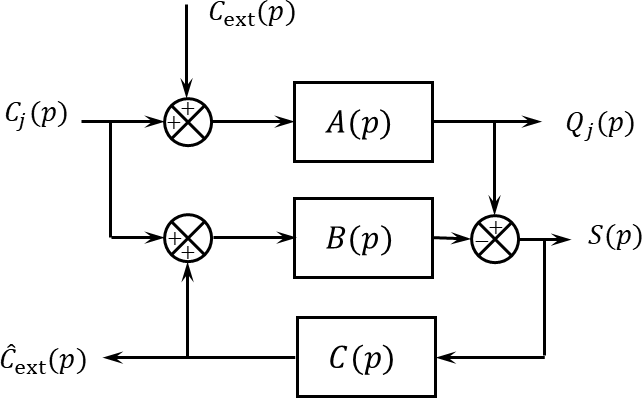
\includegraphics[width=.4\linewidth]{images/fig_04}
\end{center}

\subparagraph{}%26
On note $A(p)$, $B(p)$ et $C(p)$ les trois fonctions de transfert des trois blocs recherchés. 


On a : $Q_j(p)=A(p)\left(C_j(p)+C_{\text{ext}}(p)\right)$, 
$S(p)=Q_j(p)-B(p)\left( C_j(p)+\hat{C}_{\text{ext}}(p) \right)$
et  $\hat{C}_{\text{ext}}(p)=C(p)S(p)$.

 soit 

$\hat{C}_{\text{ext}}(p)=C(p)\left(Q_j(p)-B(p)\left( C_j(p)+\hat{C}_{\text{ext}}(p) \right)\right)$

$\Leftrightarrow \hat{C}_{\text{ext}}(p) \left(1+ C(p)B(p)\right)=C(p)\left(Q_j(p)-C(p)B(p) \right)$

Il semblerait qu'il manque une information concernant le schéma bloc. Il faudrait sans doute ajouter \^{Q}$_j(p)$. Cela donnerait directement :

\begin{center}
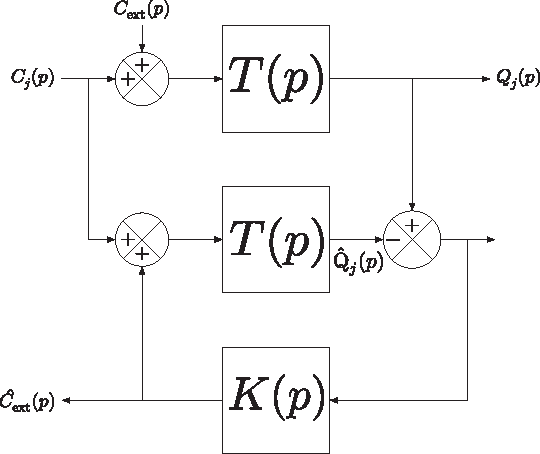
\includegraphics[width=0.7\textwidth]{images/DR_B_corrige.pdf}
\end{center}

\subparagraph{}%27

\subparagraph{}%28

\subparagraph{}%29


\section{Analyse des performances vis-à-vis des mouvements respiratoires}
\begin{obj}
Quantifier le niveau de performance de la loi de commande déterminée en considérant la consigne
correspondant aux mouvements physiologiques. Une amélioration de la loi de commande est ensuite
envisagée sous la forme d’une anticipation sur la consigne pour améliorer les performances.
\end{obj}


\subparagraph{}\textit{}%30
Pour un signal périodique en entrée d'amplitude $B$, l'écart sera un signal périodique d'amplitude $0,066B$.  Soit \SI{2,64e-3}{rad} et \SI{5,94e-3}{rad}.

\textbf{Conclure ?}

\subparagraph{}\textit{}%31
On a $C_j(p)=C_u(p)+C_a(p)$ 
$=\left(\varepsilon(p)K_1 - K_2 p Q_j(p)\right) + C_a(p) $

$=\left( \left( Q_j^\star (p)-Q_j(p)\right)K_1 - K_2 p Q_j(p)\right) + C_a(p) $

$=\left( \left( Q_j^\star (p)-Q_j(p)\right)K_1 - K_2 p C_j(p) T(p)\right) + C_a(p) $.

En considérant que  la consigne est suivie sans erreur, on a 
$C_j(p)= - K_2 p C_j(p) T(p) + C_a(p) $ et donc $C_j(p)=\dfrac{1}{1+K_2p T(p)}C_a(p)$.
\textcolor{red}{Est-ce la bonne piste ?}
\subparagraph{}\textit{}%32
%% $K_a(p)$ = ??

On a $Q_j(p) = C_j(p) T(p)= \left( Q_j^{\star}(p) K_a(p) + C_u(p) \right) T(p)$
$= \left( Q_j^{\star}(p) K_a(p) + C_u(p) \right) T(p)$
$= \left( Q_j^{\star}(p) K_a(p) + \left( \varepsilon(p) K_1 - K_2 p Q_j(p) \right)\right) T(p)$
$= \left( Q_j^{\star}(p) K_a(p) + \left( \left(Q_j^{\star}(p) - Q_j(p) \right) K_1 - K_2 p Q_j(p) \right)\right) T(p)$

%$Q_j(p) = \left( Q_j^{\star}(p) K_a(p) + \left( \left(Q_j^{\star}(p) - Q_j(p) \right) K_1 - K_2 p Q_j(p) \right)\right) T(p)$

$\Leftrightarrow Q_j(p) = 
\left(
    Q_j^{\star}(p) K_a(p) + 
    \left( 
        \left(Q_j^{\star}(p) - Q_j(p) \right) K_1 - K_2 p Q_j(p) 
    \right)
\right) T(p)$

$\Leftrightarrow Q_j(p) = 
    T(p)Q_j^{\star}(p) K_a(p) + 
    T(p)\left( 
        \left(Q_j^{\star}(p) - Q_j(p) \right) K_1 - K_2 p Q_j(p) 
    \right) $

$\Leftrightarrow Q_j(p) = 
    T(p)Q_j^{\star}(p) K_a(p) + 
        T(p)K_1 Q_j^{\star}(p) -T(p)K_1  Q_j(p)   - T(p)K_2 p Q_j(p) 
     $

$\Leftrightarrow Q_j(p)\left(1     +T(p)K_1     + T(p)K_2 p\right)= 
      Q_j^{\star}(p)T(p) \left(  K_a(p)     +K_1 \right)     $

On a donc $F(p)=\dfrac{Q_j(p)}{Q_j^{\star}(p)}=\dfrac{ K_a(p) +K_1}{1+T(p)K_1 + T(p)K_2 p}$.


\subparagraph{}\textit{}%33

\subparagraph{}\textit{}%34

\end{document}
\begin{center}
\includegraphics[width=\linewidth]{images/img_04}
%\textit{}
\end{center}



